%Präambel:
\documentclass{article}						% Vor dem Drucken auf scrartcl ändern
\usepackage[ngerman]{babel}
\usepackage[utf8]{inputenc}					% für Sonderzeichen
\usepackage[T1]{fontenc}					% zur Umsetzung von Sondereichen
\usepackage{url}
\usepackage[pdfborder ={0 0 0}]{hyperref}	% für Verlinkungen
\usepackage{enumitem}						% Zum Nummerieren
\usepackage{amsmath}						% Math. Zeichen
\usepackage{amssymb}						% Math. Symbole
\usepackage{graphicx}						% Bilder einfügen
\usepackage{longtable}						% Tabellen über eine Seite
\usepackage{subfigure}						% Zwei Bilder nebeneinander
\usepackage{wrapfig}
\usepackage{caption}						% Hilfsmittel, damit Bilder nicht auf die nächste Seite geschoben werden
\usepackage[decimalsymbol=comma]{siunitx}				% Für schöne Einheiten mit Komma
            


\title{Rauschgrundlagen und Verstärkerrauschen}
\author{Friedrich Möller und Wilhelm Eschen}

\begin{document}
	\maketitle
	\tableofcontents
	\clearpage
			

\section{Aufgaben}
	\subsection*{Versuchstag 1 - Rauschgrundlagen}
		
		\subsubsection*{Aufgabe 1.1 - Eigenschaften von Rauschsignalen}
			\begin{enumerate}
				\item Nehmen Sie ein Histogramm von weißem Rauschen auf.
				\item Bestimmen Sie den Mittelwert, Effektivwert sowie die Varianz eines
Rauschsignals. Vergleichen Sie mit einem aufgenommenen Spektrum.
				\item  Untersuchen Sie die Autokorrelationsfunktion von weißem Rauschen. Vergleichen
Sie die Resultate mit dem Spektrum des Signals.
				\item Wiederholen Sie die die letzten zwei Punkte nur nach Durchgang durch einen Tiefpass geeigneter Grenzfrequenz.
				\item Erzeugen Sie 3 verschiedene Signale-/Rausch-Verhältnisse und bewerten Sie das
Signal
			\end{enumerate}
			
		\subsubsection*{Aufgabe 1.2 - Rauschreduktion}
			\begin{enumerate}
				\item Wählen Sie ein SNR aus Aufgabe 1.1.5 aus und lassen Sie das Signal unterschiedlich
oft akkumulieren. Bewerten Sie das SNR nach der Akkumulation.
				\item Bestimmen Sie die Rauschbandbreite des Tiefpasses aus Aufgabe 1.1.3. Legen Sie
nun das Signal-Rausch-Gemisch aus Aufgabe 1.2.1 an den Tiefpass an und
bewerten Sie das SNR nach dem Durchgang durch den Filter. Vergleichen Sie mit
den theoretischen Vorhersagen.
				\item Bewerten Sie das Signal vor und nach dem Durchgang durch einen Schmalbandverstärker.
\end{enumerate}		

	\subsection*{Versuchstag 2 - Verstärkerrauschen}
		\subsubsection*{Aufgabe 1.1 - Verstärkereigenschaften}
			\begin{enumerate}
				\item Bestimmen Sie die Amplitudenübertragungsfunktion der vorliegenden
Verstärkerschaltung.
				\item Bestimmen Sie aus den Daten aus Aufgabe 1a) das Verstärkungs-Bandbreite-
Produkt. 
				\item Bestimmen Sie die Offsetspannung des Verstärkers.
			\end{enumerate}	
		\subsubsection*{Aufgabe 1.2 - Störungen}
			\begin{enumerate}
				\item Vergleichen Sie das Verhalten einer hochohmigen sowie einer niederohmigen
Quelle.
				\item Untersuchen Sie das Störspektrum bei hochohmigen Eingang.
				\item Untersuchen Sie die Wirkung einer Abschirmung.
			\end{enumerate}
		\subsubsection*{Aufgabe 1.3 - Verstärkerrauschen}
			\begin{enumerate}
				\item Nehmen Sie das Rauschspektrum des vorliegenden Verstärkers auf und
bestimmen Sie den Abknickpunkt des 1/f-Rauschens.
				\item Bestimmen Sie die Rauschparameter des vorliegenden Verstärkers für das
einfache Verstärkerrauschmodell.
				\item Wie groß muss der Innenwiderstand der Signalquelle gewählt werden, um Rauschanpassung zu erhalten?
			\end{enumerate}				
\clearpage

\section{Grundlagen}
				\subsection{Rauschgrundlagen}
			Rauschen ist die statistische Schwankung einer Messgröße. Dieser Vorgang kommt durch Zitterbewegung von Ladungsträgern zustande und überlagert somit jede Messung bei $T \neq 0 \ K$. Empfindliche Messungen laufen daher am Rauschlimit.
			Zur Charakterisierung von Rauschen eignet sich die Varianz:
			\begin{equation}
				\left\langle U^{2} \right\rangle = \frac{1}{T} \int\limits_{0}^{T} \left(U(t)- \langle U \rangle \right)^{2} \operatorname{d}t \ .
			\end{equation}
			Für eine bessere Vergleichbarkeit mit den Amplituden verwendet man oft auch die Standardabweichung:
			\begin{equation}
				\sqrt{\left\langle U^{2} \right\rangle} = \sqrt{\frac{1}{T} \int\limits_{0}^{T} \left(U(t)- \langle U \rangle \right)^{2} \operatorname{d}t} \ .
			\end{equation}
			Der Mittelwert hingegen eignet sich nicht zur Charakterisierung des Rauschens, da sich im Mittel gleich viele positive, wie negative Werte ergeben.
			\begin{equation}
				\left\langle U \right\rangle = \frac{1}{T} \int\limits_{0}^{T} U(t) \operatorname{d}t =0 \ .
			\end{equation}
		\newline
		Rauschprozesse werden hinsichtlich Ihres Spektrums unterteilt. Die häufigsten auftretenden Rauscharten sind:
		\begin{itemize}
			\item weißes Rauschen: konstantes Frequenzspektrum
			\item rosa Rauschen: niedrige Frequenzen stärker vertreten als hohe: $F(\omega) \propto \frac{1}{\omega ^{n}}$ mit $n=1\cdots 2$
			\item thermisches Rauschen: $U_n ^2=4k_{B}TR\Delta f$
		\end{itemize}
		Eine wichtige Größe für die Beschreibung des Elektronischen Rauschen, welches ein zu messendes Signal überlagert, ist das Signal-Rausch-Verhältnis (SNR). Es gilt:
		\begin{equation}
			SNR=\frac{P_{Signal}}{P_{Rauschen}}=\frac{\frac{U_{Signal}^2}{R}}{\frac{U_{Rauschen}^2}{R}}=\frac{U_{Signal}^2}{U_{Rauschen}^2}
		\end{equation}
		Hierbei gilt das zweite Gleichheitszeichen nur, wenn  Signal und Rauschen an einem Ohmschen Widerstand abgegriffen werden. Dabei gilt $U_{Rauschen}^2=\left\langle U_{Rauschen}^{2} \right\rangle$. Bei Rauschen in zusammengesetzten Systemen erfolgt die Addition der Rauschleistungen, nicht der Amplituden: $U_{ges}^2=U_1^2+U_2^2$ .
		\newline
		Beim zweiten Versuchsteil sollte die Reduktion des Rauschens, also die Verbesserung des SNR untersucht werden. Dabei ist eine Möglichkeit die Akkumulation. Dies ist das wiederholte Aufaddieren des Signal Rausch Gemischs und anschließende Division durch die Anzahl der Prozesse. 
		Dadurch verringert sich das Rauschen mit $1/\sqrt{N}$ durch den Mittelungsprozess- das Signal bleibt erhalten, wenn phasenrichtige Addition garantiert ist.
		Mittels der Autokorrelationsfunktion, welche gemäß 
		\begin{equation}
			AKF(\tau)=\lim_{T \rightarrow \infty} \frac{1}{2T} \int \limits_{-T}^{+T} U(t) \cdot U(t+\tau) \operatorname{d}t
		\end{equation}
		definiert ist, kann die Periode des Signals im Signal-Rausch-Gemisch bestimmt werden. Dies funktioniert da für ein periodisches Signal die Anwendung der AKF die Periode erhalten lässt. Dadurch wird gezieltes Filtern möglich.
		Ebenfalls kann mittels Filtern (Tiefpass, Hochpass oder Bandpass) das Rauschen weit weg vom Signal gezielt gedämpft werden.
		
	\subsection{Verstärkerrauschen}
		Zunächst sollte man zu unterscheiden wissen, ob ein Rauschen, oder eine Störung vorliegt. Per Definition sind Störungen extern aufgeprägte, und dadurch abschirmbare unerwünschte Signale.
		Rauschen hingegen sind intrinsisch, als stets vorhandene, jedoch optimierbare, unerwünschte Signale.
		Störungen können Elektromagnetische Einstrahlungen oder beispielsweise magnetische Einkopplungen sein, welche durch Faraday-Käfig bzw. ferromagnetische Umhausung abgeschirmt werden können.
		\newline
		 Verstärker dienen der Anhebung der Signalamplitude. Dabei tritt thermisches Rauschen in allen Komponenten auf. Ein Verstärker fügt jedem Signal-Rausch Gemisch sein Eigenrauschen hinzu.
		 Das Gesamtrauschen des Verstärkers kann durch nachfolgendes Modell dargestellt werden:
		 \begin{figure}[h!]
		 	\centering
		 	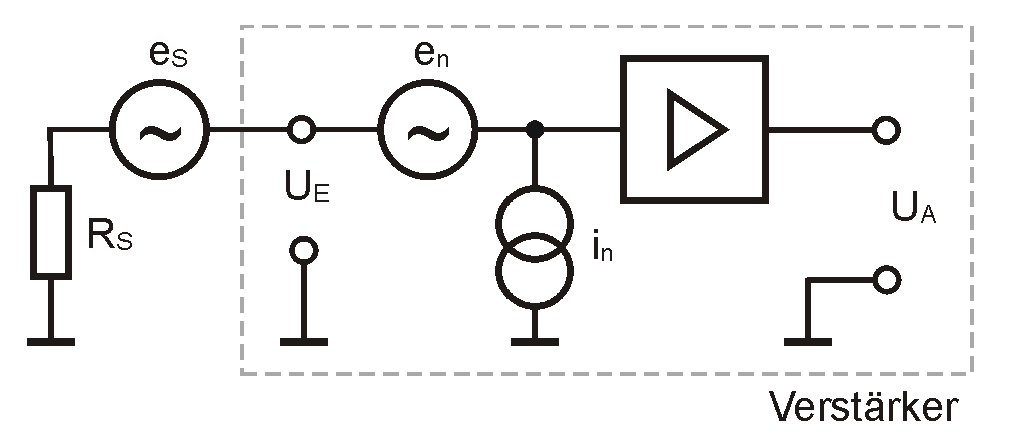
\includegraphics[scale=0.5]{GrundlagenVerstaerkermodell}
		 	\caption{Einfaches Modell für Gesamtrauschen des Verstärkers}
		 \end{figure}
		 
		 Dabei ist $R_{S}$ der angeschlossene Quellwiderstand mit dessem thermischen Eigenrauschen $e_{S}^2=4k_{B} TR_{S} \Delta f$, Eingangsspannungsrauschen $e_{n}$ und Eingangsstromrauschen $i_{n}$. Hierbei ist $k_{B} $ die Boltzmann Konstante, T die Temperatur und $\Delta f$ die Mess-oder Rauschbandbreite. Daraus ergibt sich am Ausgang die Bilanz:
		 \begin{equation}
		 	U_{A}^2=V^2 \left( e_{S}^2+e_{n}^2+R_{S}^2i_{n}^2 \right)
		 \end{equation}
		 Eine typische Abhängigkeit des Rauschens eines Verstärkers unter dem Quellwiderstand $R_{S}$ ist nachfolgend dargestellt.
		 \begin{figure}[h!]
		 	\centering
		 	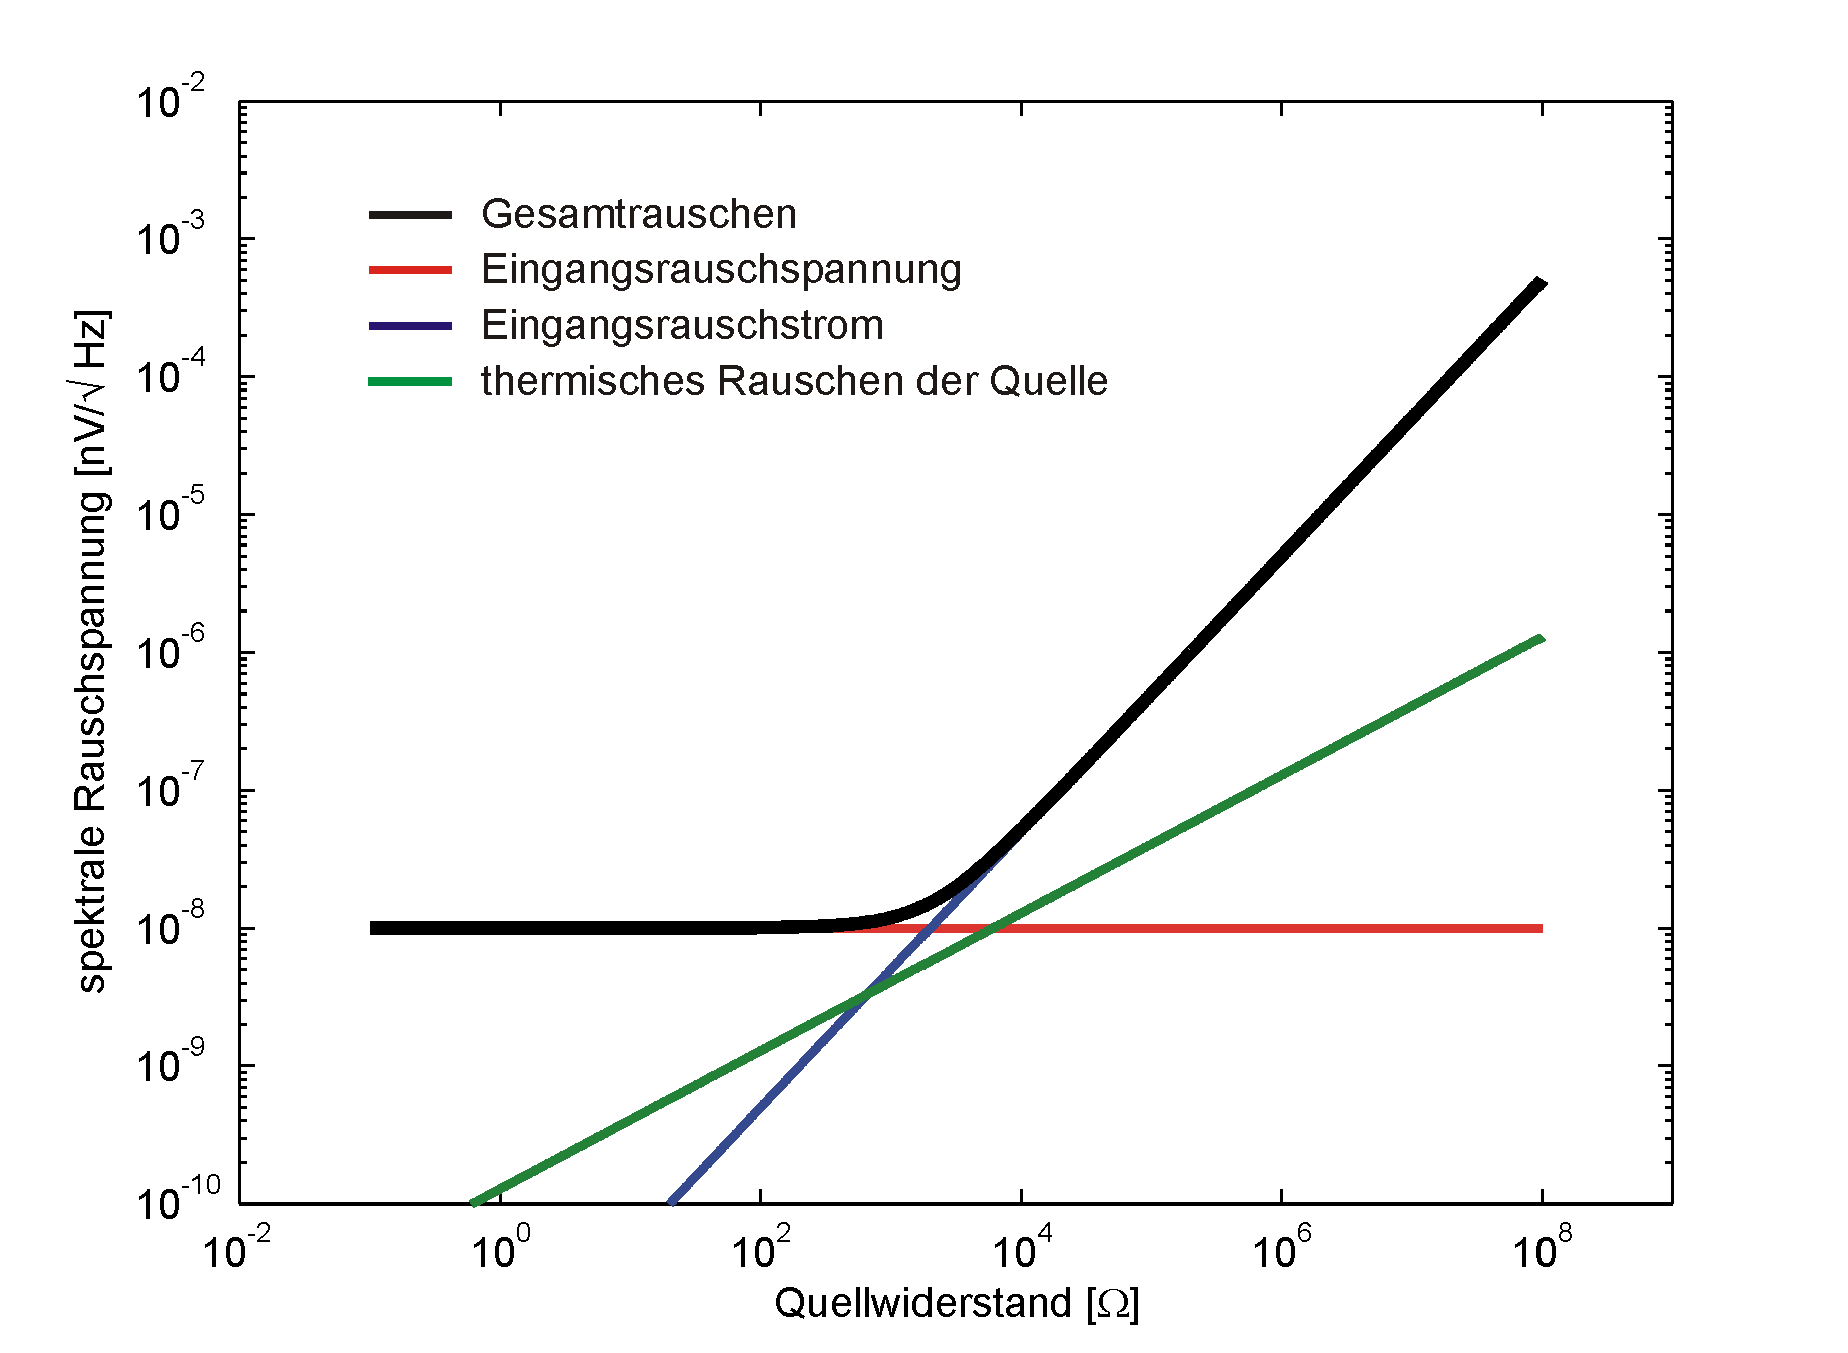
\includegraphics[scale=0.3]{Verstaerkerrauschen}
		 	\caption{Verstärkerrauschen in Abhängigkeit des Quellwiderstandes}
		 \end{figure}
		 \newline
		 Für niederohmige Quellwiderstände dominiert die Eingangsrauschspannung, für hochohmige der Eingangsrauschstrom. 
		 Parameter des Verstärkerrauschens ist die Rauschzahl $F=SNR_{Eingang}/SNR_{Ausgang}>0$ für realen Verstärker. Für die Angabe im dB-Maß ist hierbei der Vorfaktor 10, nicht 20 zu wählen, da sich die SNR auf Signal- und Rauschleistungen beziehen. Rauschanpassung liegt vor, wenn der Verstärker der Quelle die minimale Menge an Zusatzrauschen hinzufügt: $R_{opt}=\frac{e_{n}}{i_{n}}$.
\clearpage
				 
\section{Auswertung}
	\subsection{Auswertung Rauschgrundlagen}
		Zunächst sollte in Aufgabe 1.1 a) die Eigenschaften von Rauschsignalen untersucht werden. Dabei sollte zuerst ein Histogramm von weißem Rauschen erstellt werden. Es wurden dabei Histogramme aufgenommen für unterschiedlich eingestellte Offset Werte. Das Rauschen wurde auf \SI{5}{\volt}$_{PP}$ eingestellt. Wie man erkennen kann, entspricht der Offset dem Mittelwert des Rauschen. Des weiteren wurde festgestellt, dass das Histogramm einer Normalverteilung entspricht.
		
		\begin{figure}[h!]
			\subfigure[Zeitverlauf Offset = \SI{0}{\volt}]{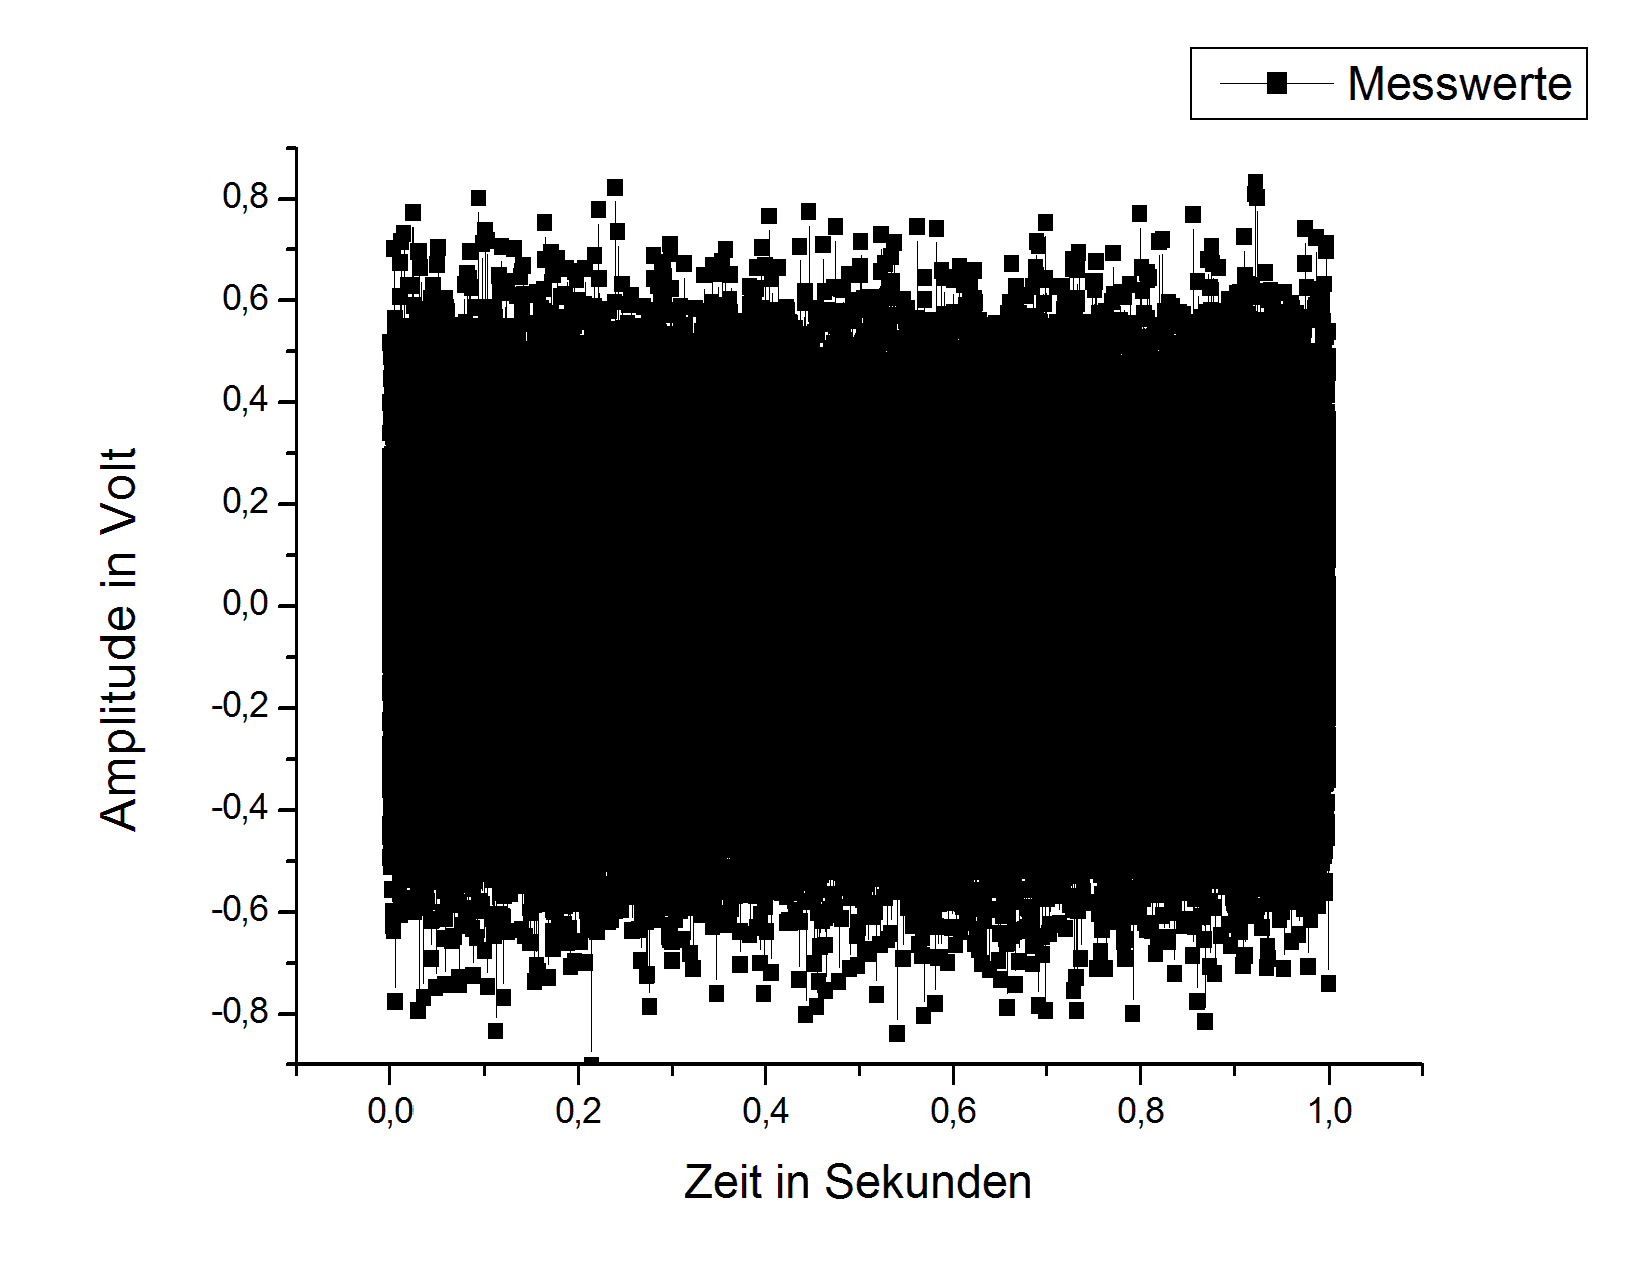
\includegraphics[scale=0.25]{1,1_a_V_Offset_5VPP_Zeit.png}}
			\subfigure[Histogramm Offset = \SI{0}{\volt}]{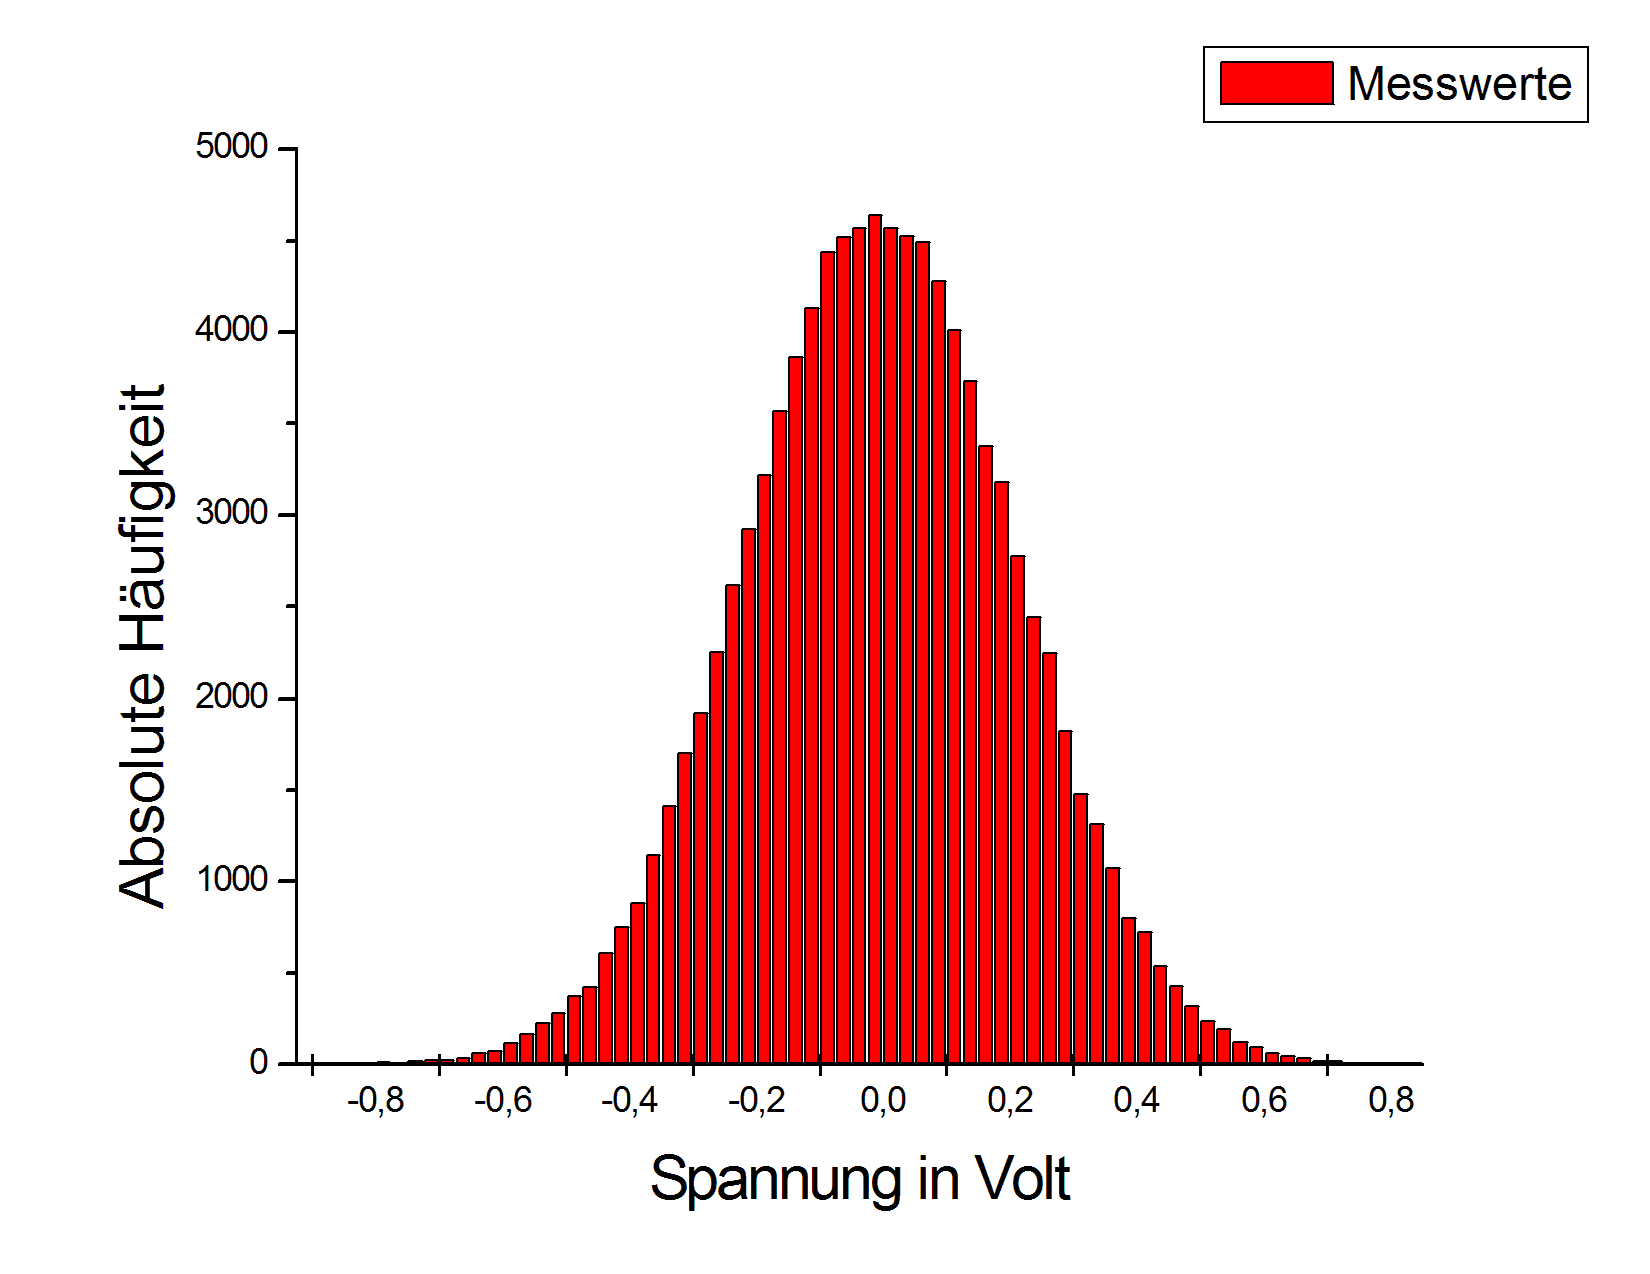
\includegraphics[scale=0.25]{1,1_a_0V_Offset_5VPP_Histo}}
		\end{figure}
		
		\begin{figure}[h!]
			\subfigure[Histogramm Offset = \SI{500}{\milli\volt}]{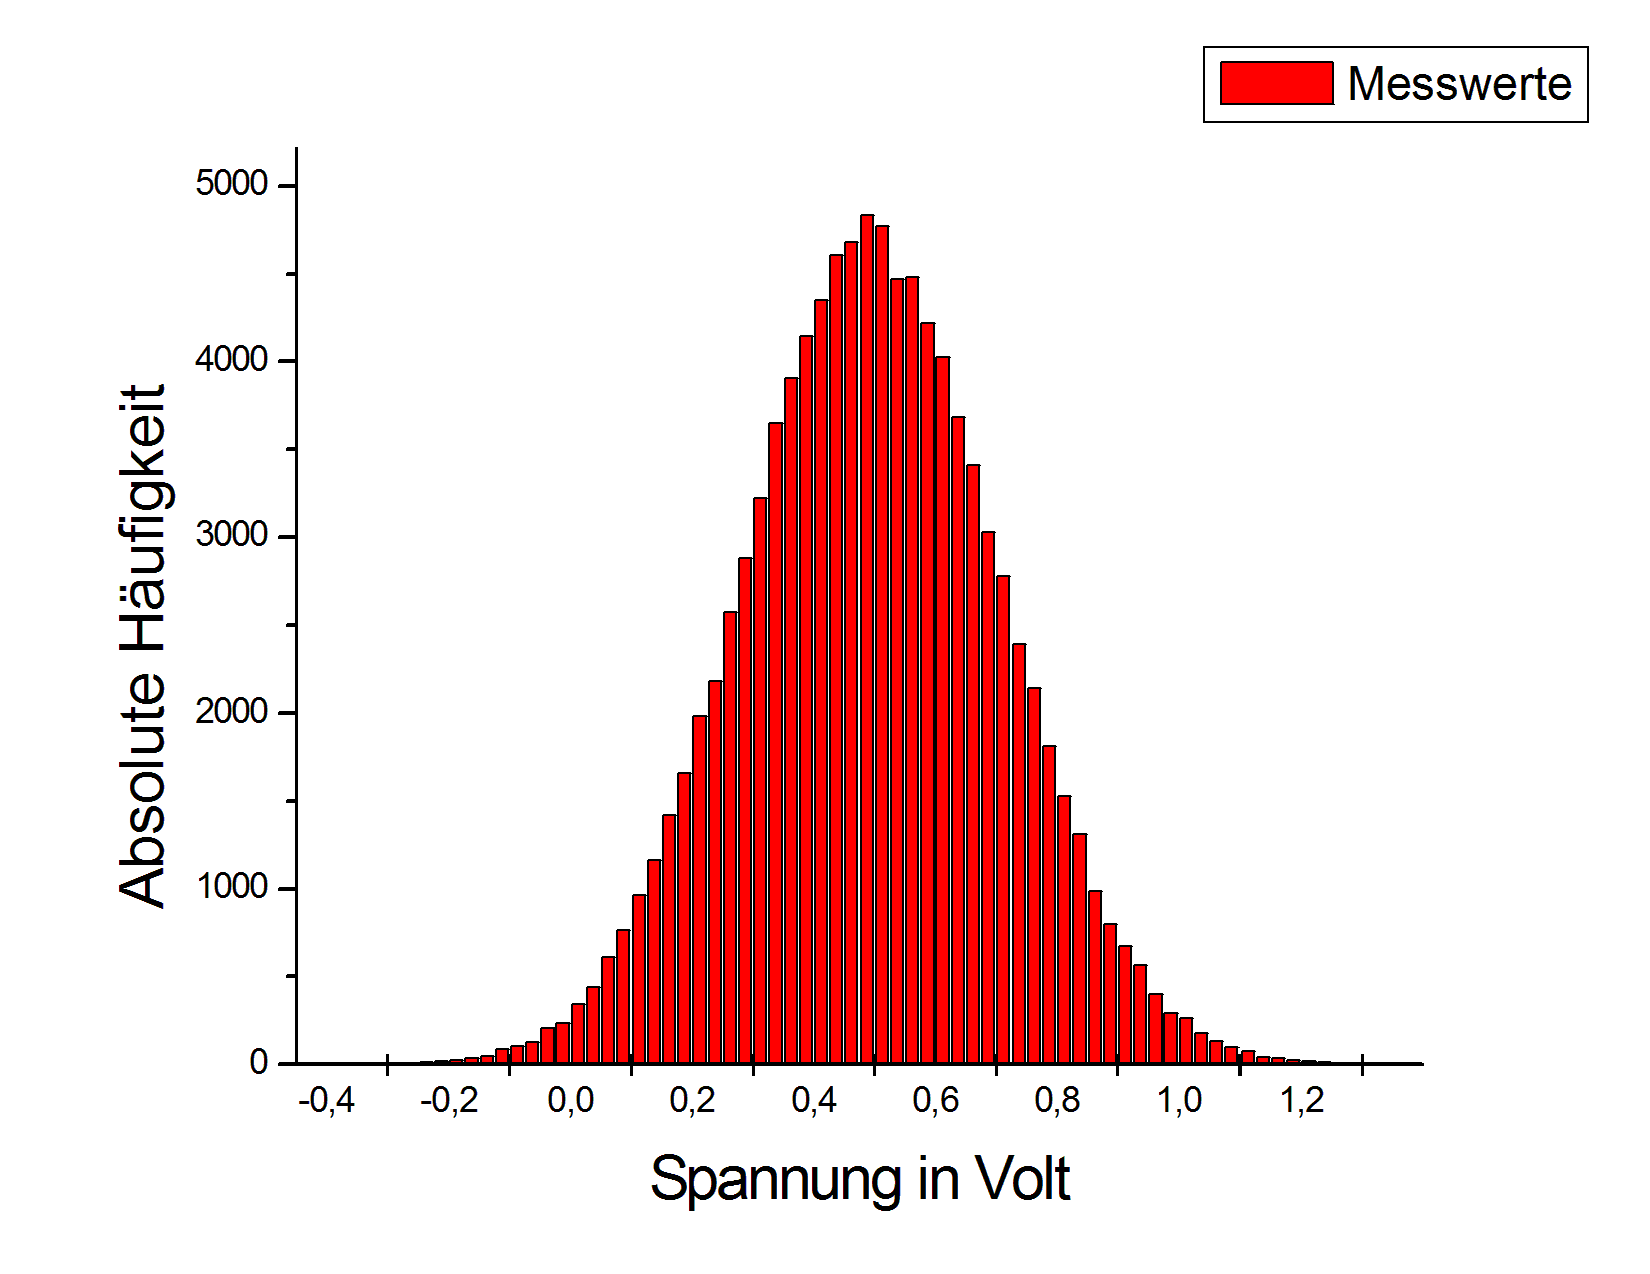
\includegraphics[scale=0.25]{1,1_a_500mV_Offset_5VPP_Histo}}
			\subfigure[Histogramm Offset = \SI{1}{\volt}]{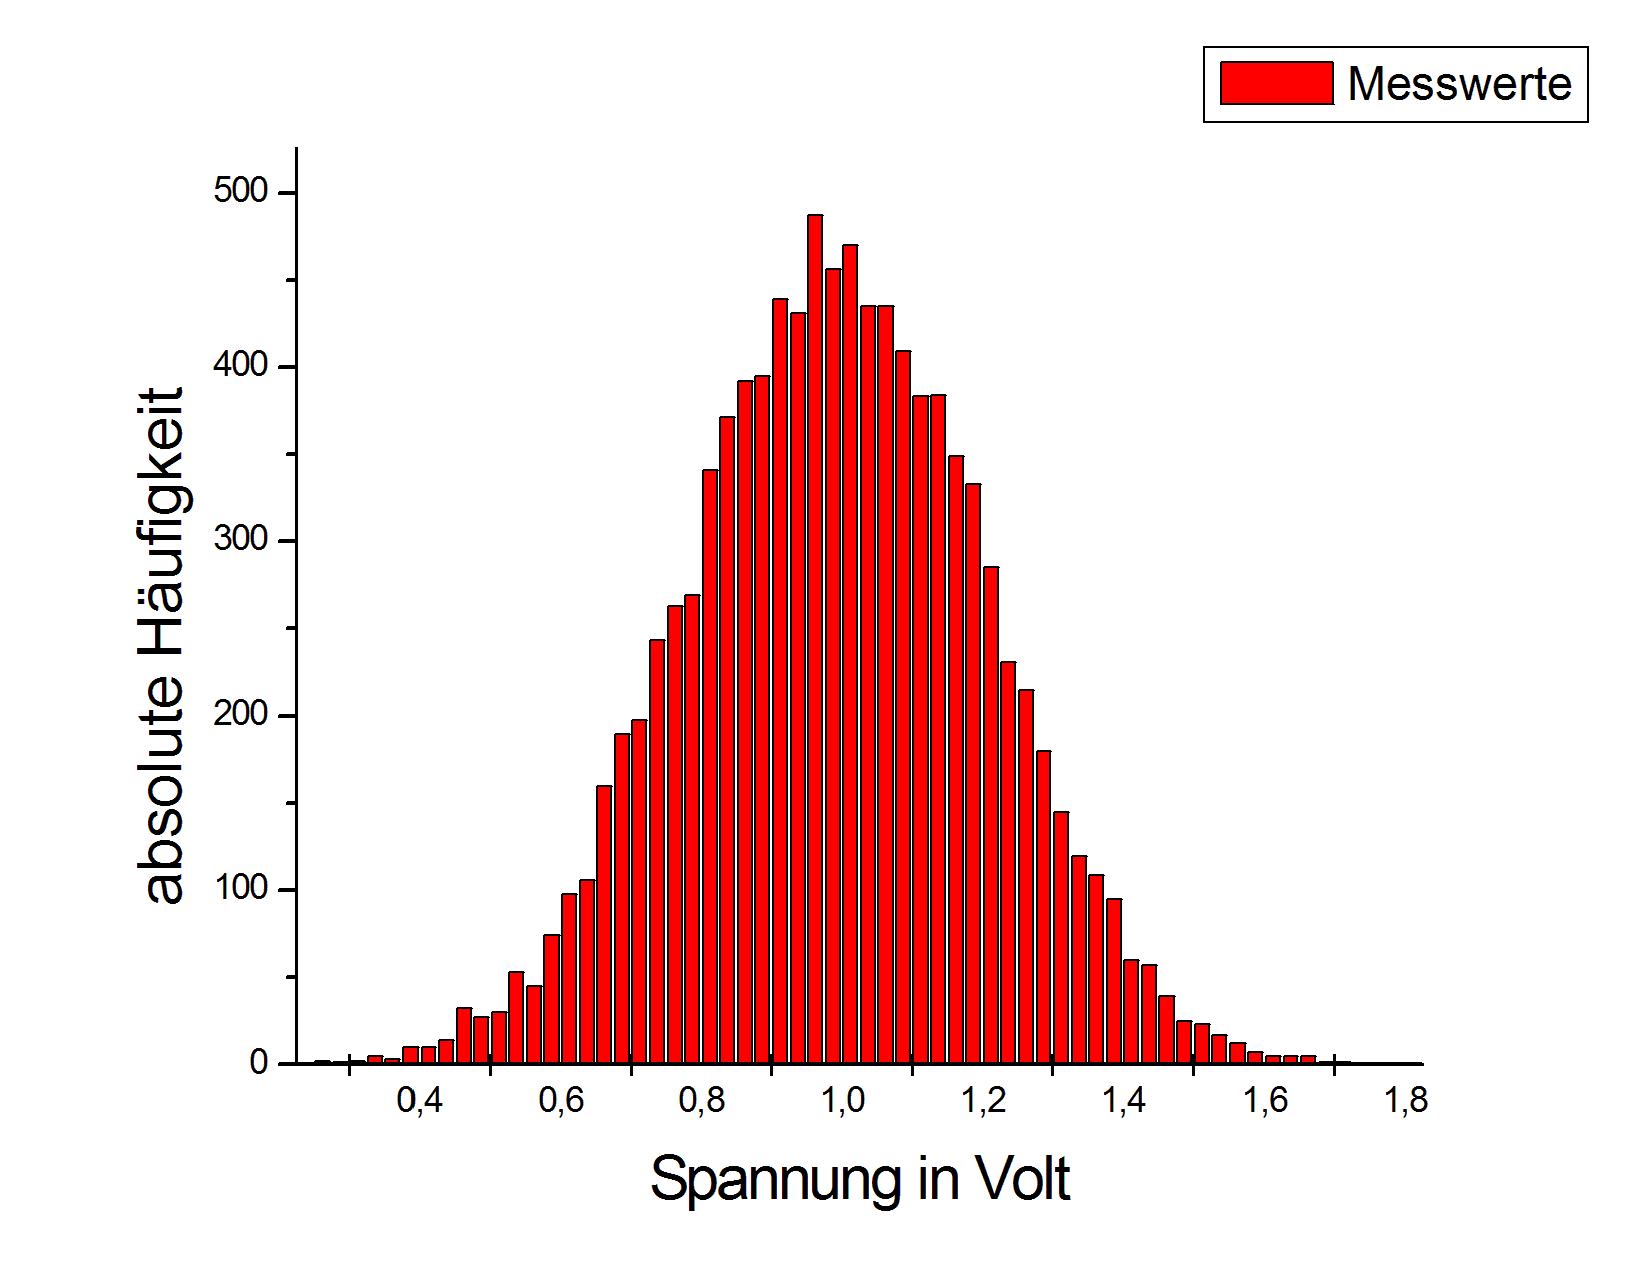
\includegraphics[scale=0.25]{1,1_a_1V_Offset_5VPP_Histo}}
		\end{figure}
		
		In Aufgabe 1.1 b) sollte danach der Mittelwert, Effektivwert und Varianz vom Rauschen bestimmt werden. Dafür wurden zunächst ein Offset von $ U_{Offset} = \SI{0,5}{\volt} $ verwendet und folgende Werte notiert. \\
		\begin{center}
			\begin{tabular}{|c|c|}
			\hline Mittelwert & $ \SI{0,495}{\volt} $ \\ 
			\hline Effektivwert & $ \SI{0,215}{\volt} $ \\ 
			\hline Varianz & $ \SI{0,046}{\volt^2} $ \\ 
			\hline 
			\end{tabular} 
		\end{center}
		
		Der Mittelwert konnte durch das Einstellen des Offset-Werts verändert werden. Durch eine Änderung der Rauschamplitude konnte die Amplitude des Rauschen verringert werden und damit die Standardabweichung und Varianz. Dies kann man im Spektrum erkennen.
		Im Spektrum kann man jedoch leider nicht erkennen, dass der Offset der Frequenz bei $ \approx \SI{0}{\hertz} $ entspricht, da diese Frequenz leider nicht mit abgespeichert wurde.
		
		\begin{figure}[h!]
			\subfigure[Spektrum $ \SI{5}{\volt_{PP}} $]{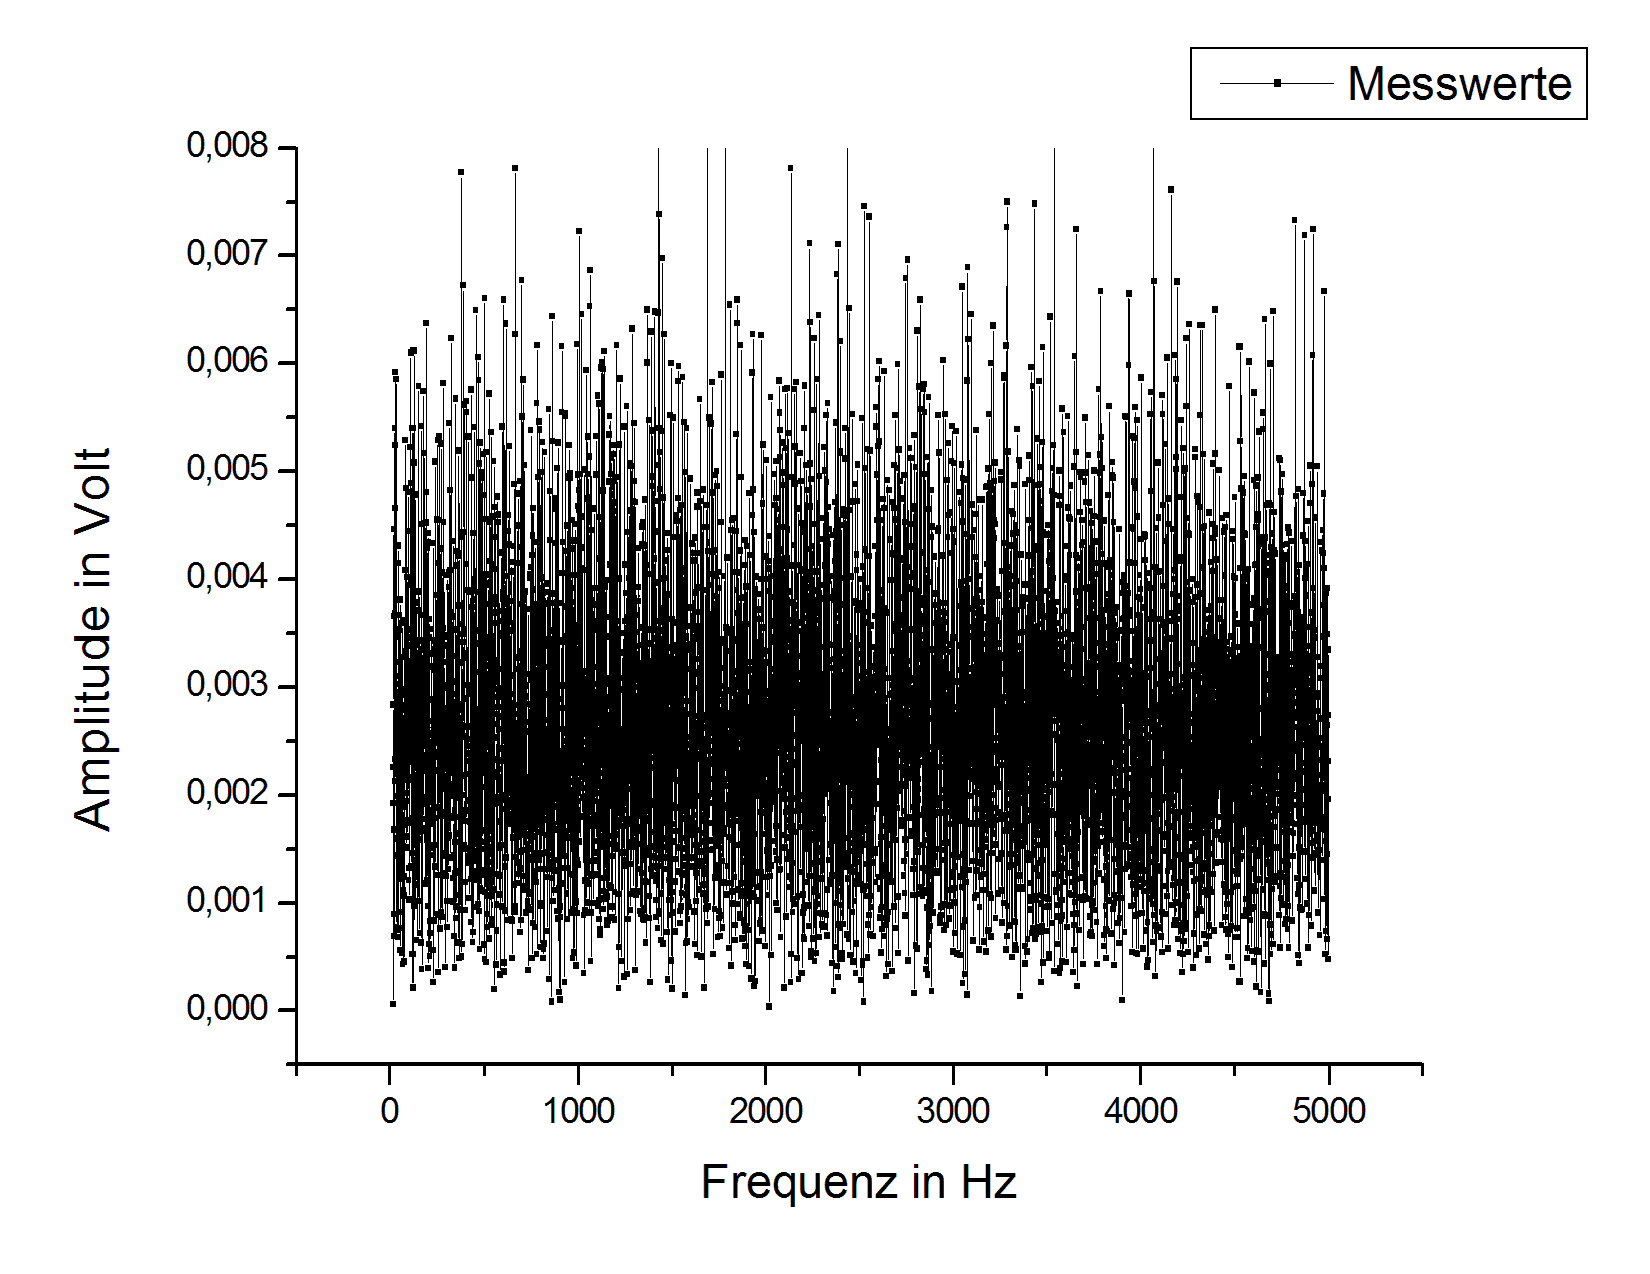
\includegraphics[scale=0.25]{1_1_b_Spektrum}}
			\subfigure[Spektrum $ \SI{500}{\milli\volt_{PP}} $]{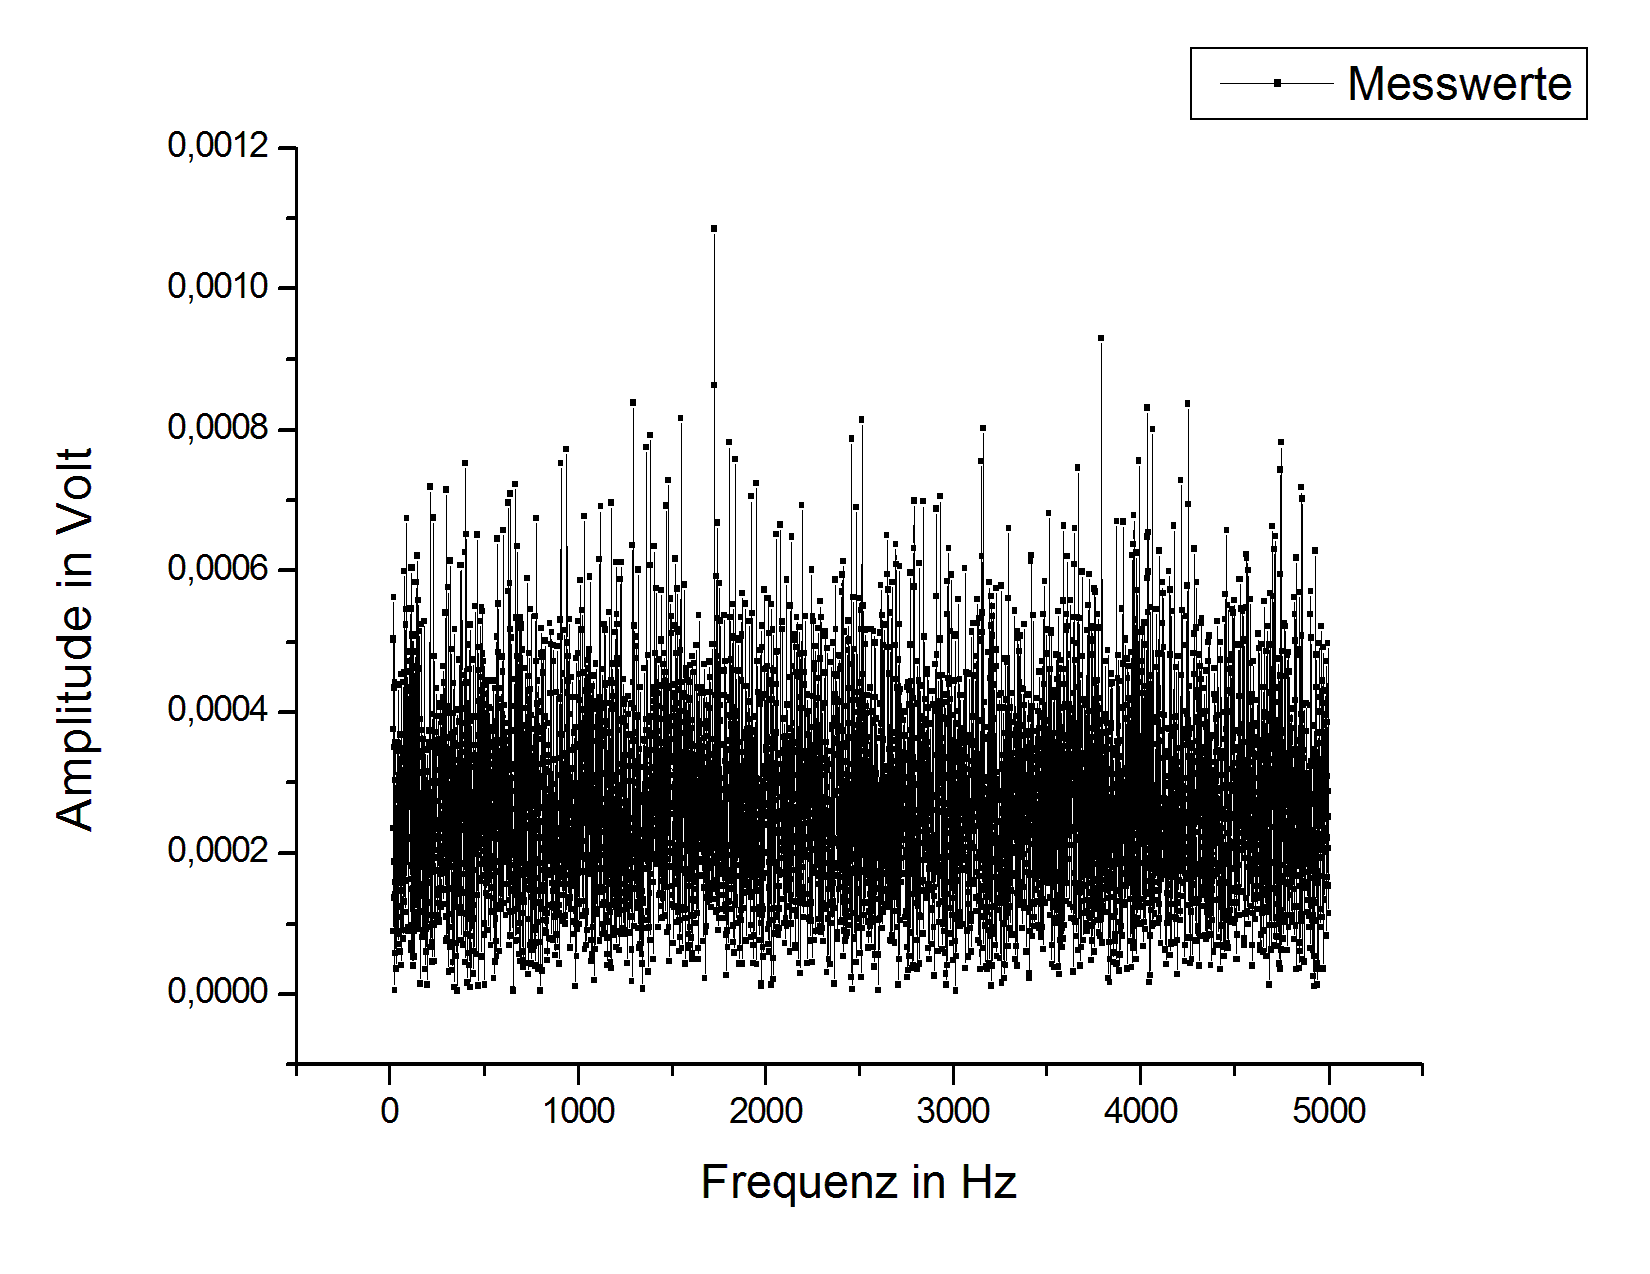
\includegraphics[scale=0.25]{1_1_b_Spektrum_0,5Vpp}}
		\end{figure}
		
		Im Aufgabenteil 1.1 c) sollte die Autokorrelationsfunktion des weißen Rauschen untersucht und mit dem Spektrum verglichen werden. Für die Autokorrelationsfunktion von weißem Rauschen wurde ein Diracimplus erwartet, da weißes Rauschen unabhängig von der Zeit ist. Es wurde dabei folgende Autokorrelationsfunktion aufgenommen. Man kann dabei einen Diracpuls mit einer gewissen Breite bei t=\SI{1}{\sec} erkennen. Jedoch ist fraglich, ob die aufgenommene Autokorrelationsfunktion richtig ist, da keine Messwerte für $ x>1 $ vorhanden waren, sodass ich die Messwerte bearbeiten musste.
		\clearpage
		
		\begin{figure}[h!]
			\subfigure[Spektrum von $ U_{Of}=\SI{1}{\volt} $ und $ \SI{3}{\volt_{PP}} $]{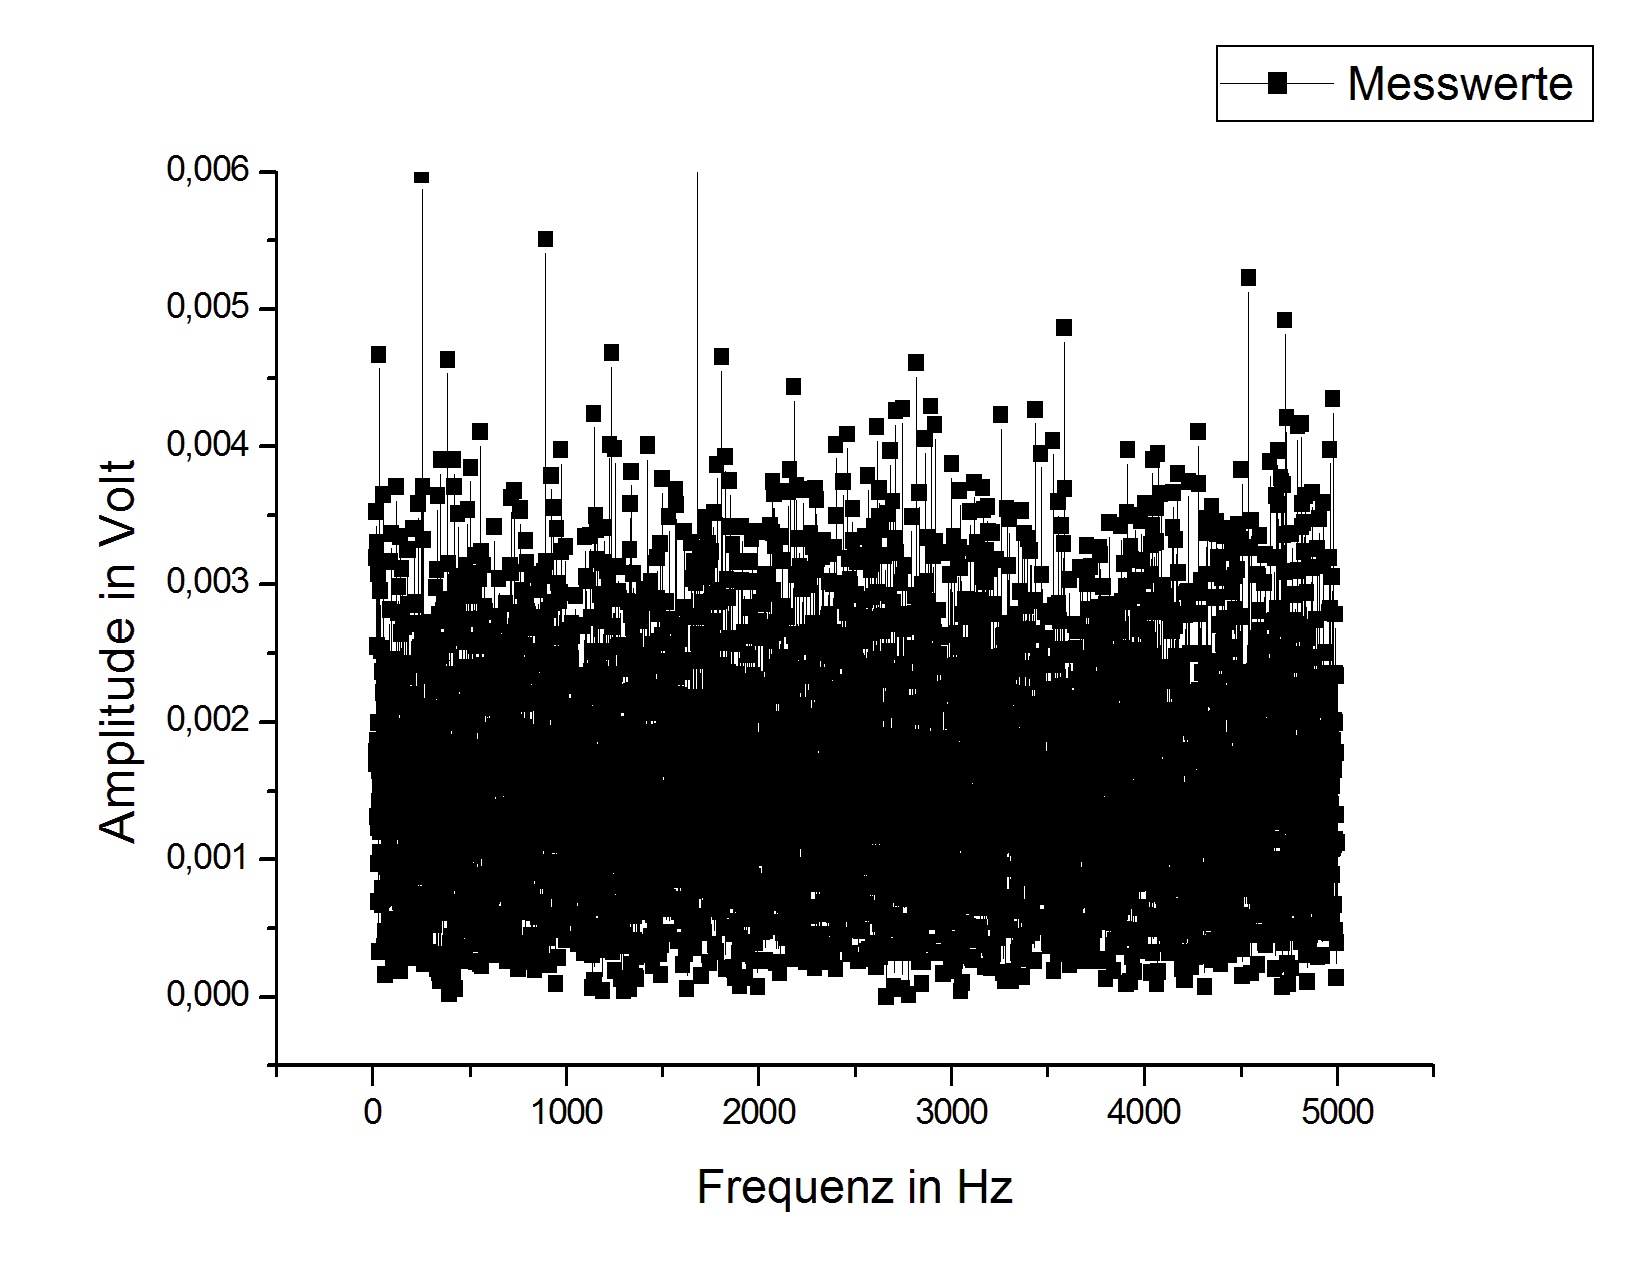
\includegraphics[scale=0.25]{Autokorrfkt_Spektrum}}
			\subfigure[Autokorrelationsfunktion von $ U_{Of}=\SI{1}{\volt} $ und $ \SI{3}{\volt_{PP}} $]{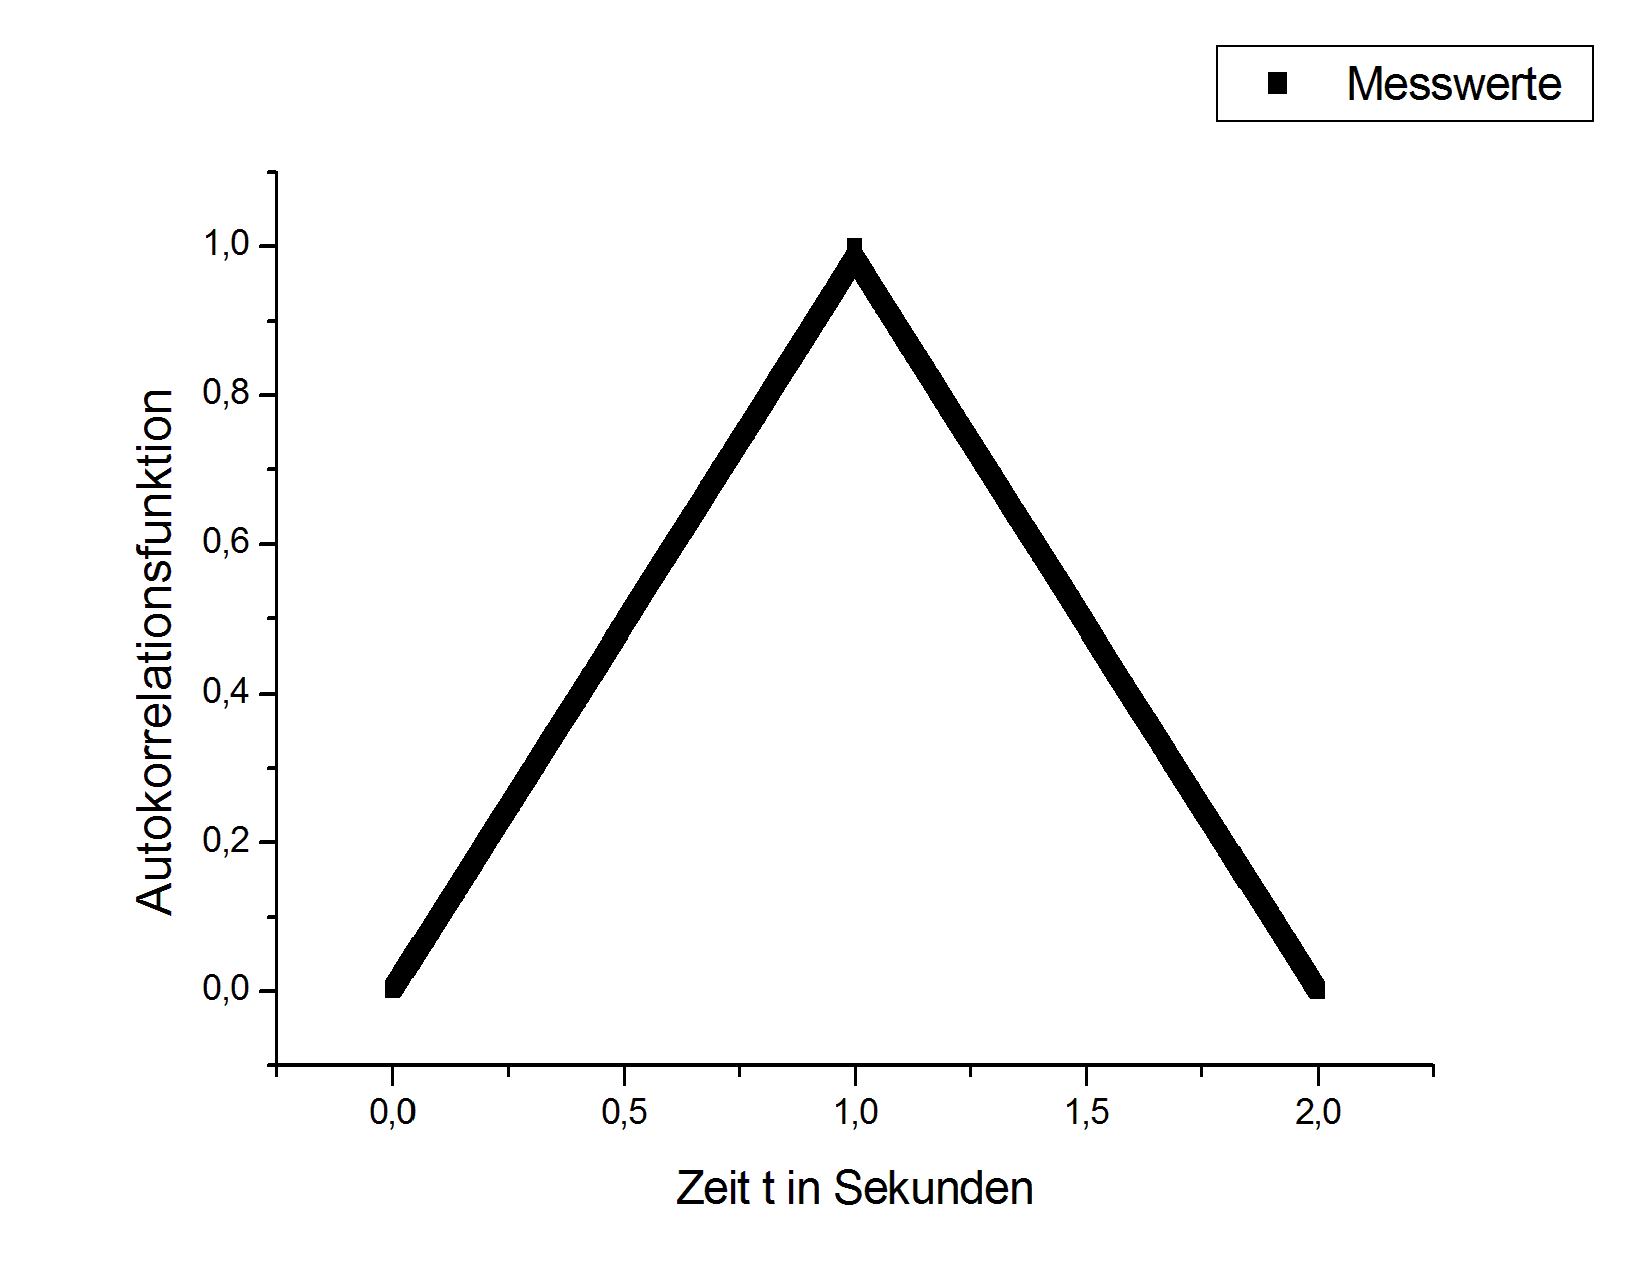
\includegraphics[scale=0.25]{AutokorrelationsFKT_1V_3Vpp}}
		\end{figure}
		
		In Aufgabe 1.1 d) sollte nun ein Tiefpass zum Filtern verwendet werden. Dabei wurde ein Widerstand von $  R = \SI{100}{\kilo\ohm} $ und ein Kondensator von $  C = \SI{100}{\nano\farad} $ gewählt. Dies ergibt $  f_{Grenz} = \frac{1}{2\pi RC} = \SI{353}{\hertz} $ Dies bestätigt die Amplitudenübertragungsfunktion. 
		
		\begin{figure}[h!]
			\centering
			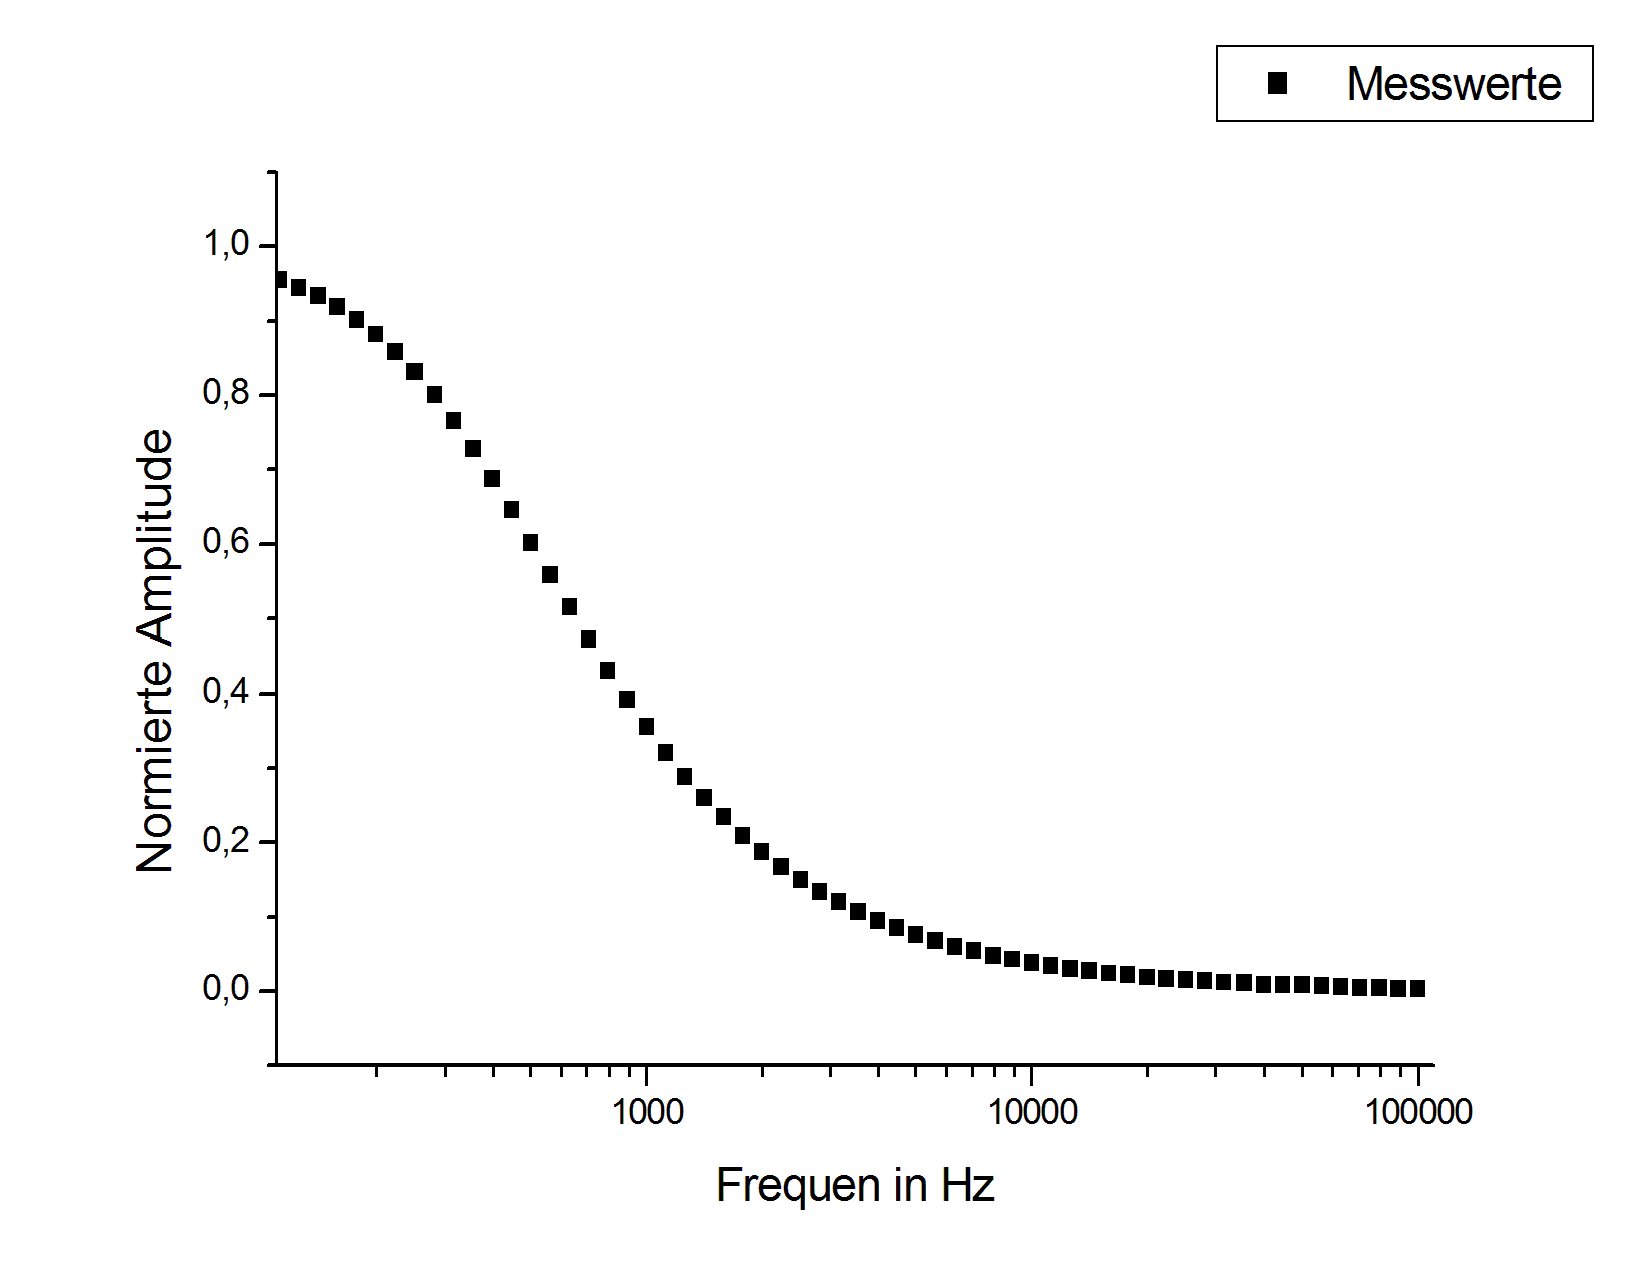
\includegraphics[scale=0.25]{Amplitudenuebertragungsfunktion}
			\caption{Amplitudenübertragungsfunktion des Tiefpasses.}
		\end{figure}
		
		Für den Mittelwert, Standardabweichung und Varianz ergeben sich folgende Werte. Wie leicht zu sehen ist, konnte durch den Tiefpass die Standardabweichung von \SI{0,215}{\volt} auf \SI{0,043}{\volt} verkleinert werde. Dies bedeutet, dass somit auch das Rauschen verringert wurde.
		\begin{center}
			\begin{tabular}{|c|c|c|}
			\hline  & Ohne Tiefpass & Mit Tiefpass \\ 
			\hline Mittelwert & \SI{0,495}{\volt} & \SI{0,501}{\volt} \\ 
			\hline Standardabweichung & \SI{0,215}{\volt} & \SI{0,043}{\volt} \\ 
			\hline Varianz & $ \SI{0,046}{\volt^2} $ & $ \SI{18}{\micro\volt^2} $ \\ 
			\hline 
			\end{tabular} 
		\end{center}

		Bei den Daten der Autokorrelationsfunktion gab es auch hier die Probleme mit den verschwunden x-Werten, die von mir hinzugefügt wurden. Im Vergleich zu der Autokorrelationsfunktion vor dem Tiefpass fällt auf, dass das Dreieck spitzer geworden ist und somit die Autokorrelationsfunktion eher dem Diracpuls ähnelt. 
		
		\begin{figure}[h!]
			\centering
			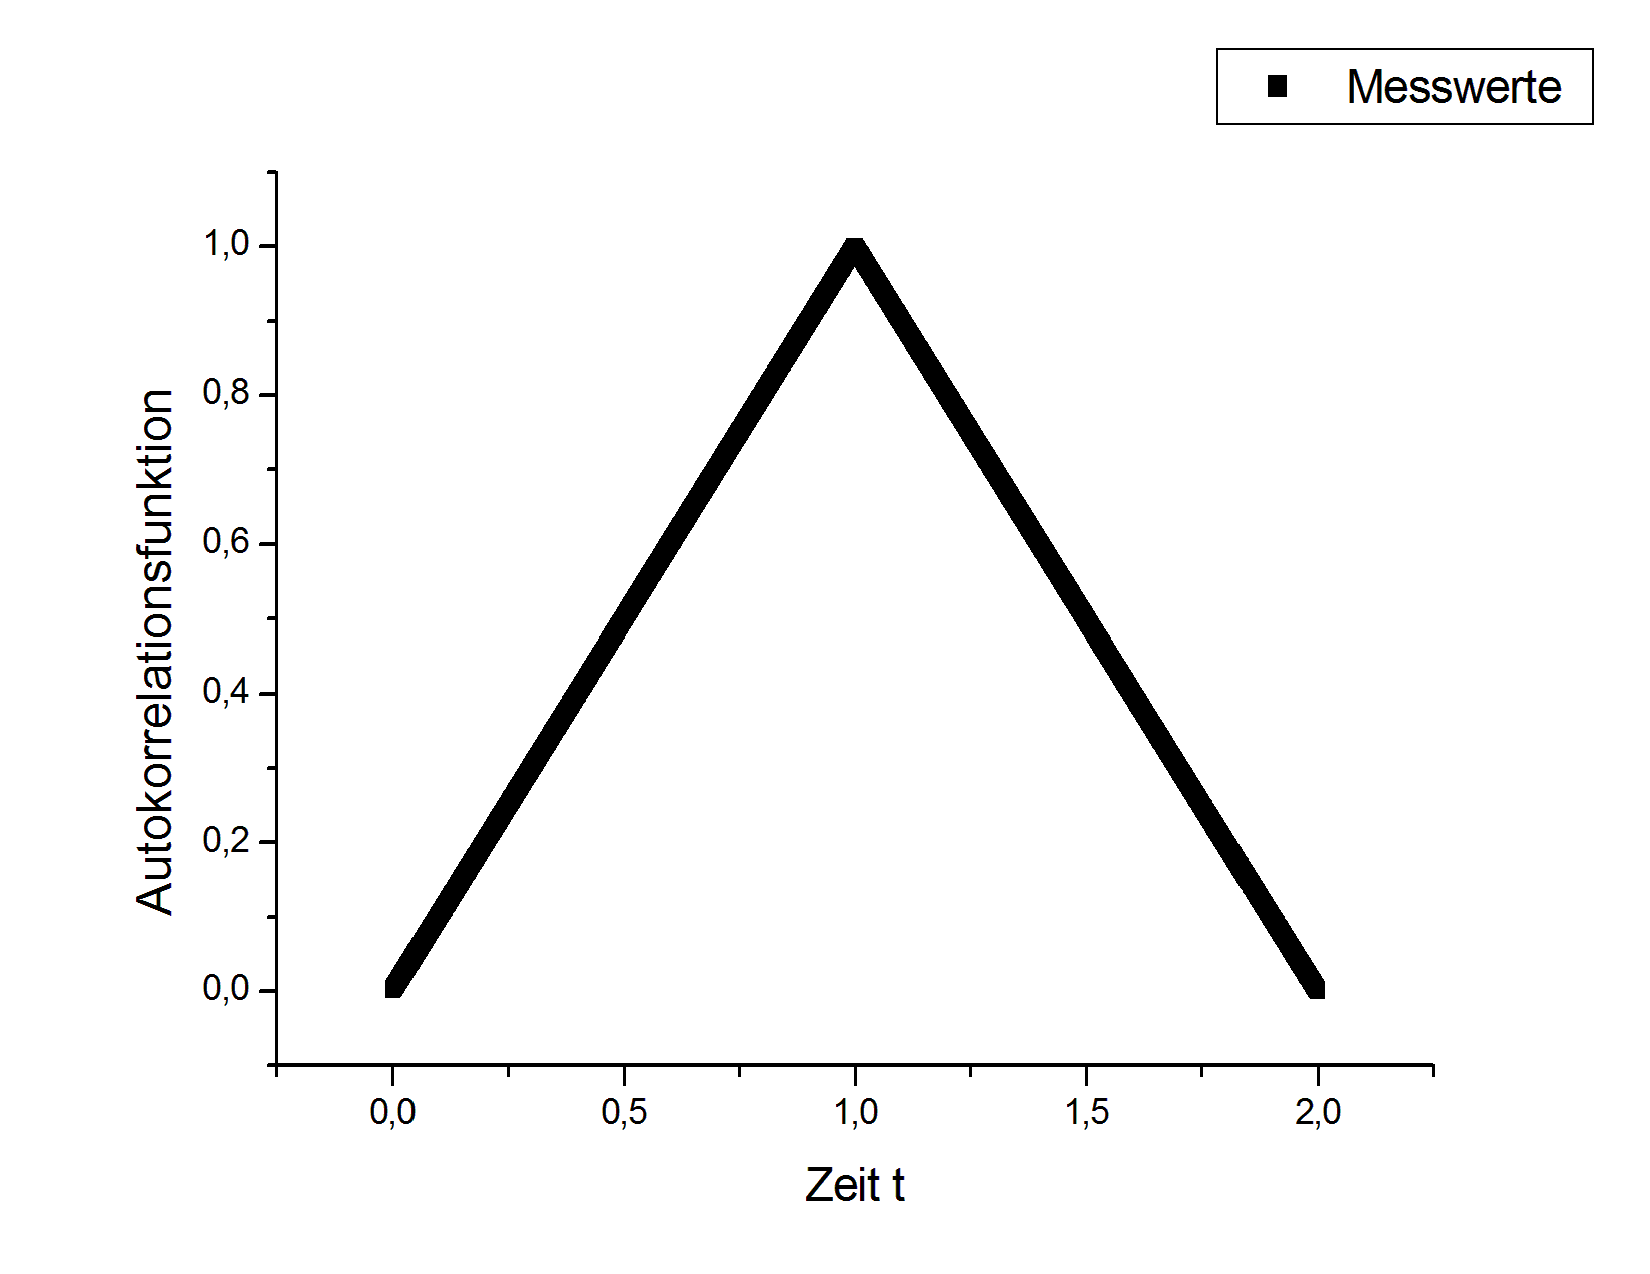
\includegraphics[scale=0.25]{TiefpasseAutokorrelationsfunktion}
			\caption{Autokorrelationsfunktion mit Tiefpass}
		\end{figure}
		
		Im Aufgabenteil 1.1 e) sollten 3 verschiedene Signal-/Rausch-Verhältnisse erzeugt werden. Als Signal wurde dabei eine Sinusspannung mit einer Frequenz von $ f = \SI{180}{\hertz} $ gewählt mit einer Amplitude von $ U = \SI{72}{\milli\volt} $. Auffallend war dabei, dass das Signal länger im Spektrum zu erkennen war als im Zeitverlauf. D.h., dass selbst bei einem $ SNR = 1,61 $ das Signal im Spektrum noch leicht zu erkennen war. Das Signal-/Rausch-Verhältnisse wurde durch $ SNR = \frac{U^2_{Signal}}{U^2_{Rausch}}$ berechnet, wobei $ U^2_{Rausch}  $ der Varianz entspricht.
		
		\begin{figure}[h!]
			\caption{SNR=640}
			\subfigure[Zeitverlauf für $ U_{Rausch}^2 = $ \SI{8,1}{\milli\volt^2}]{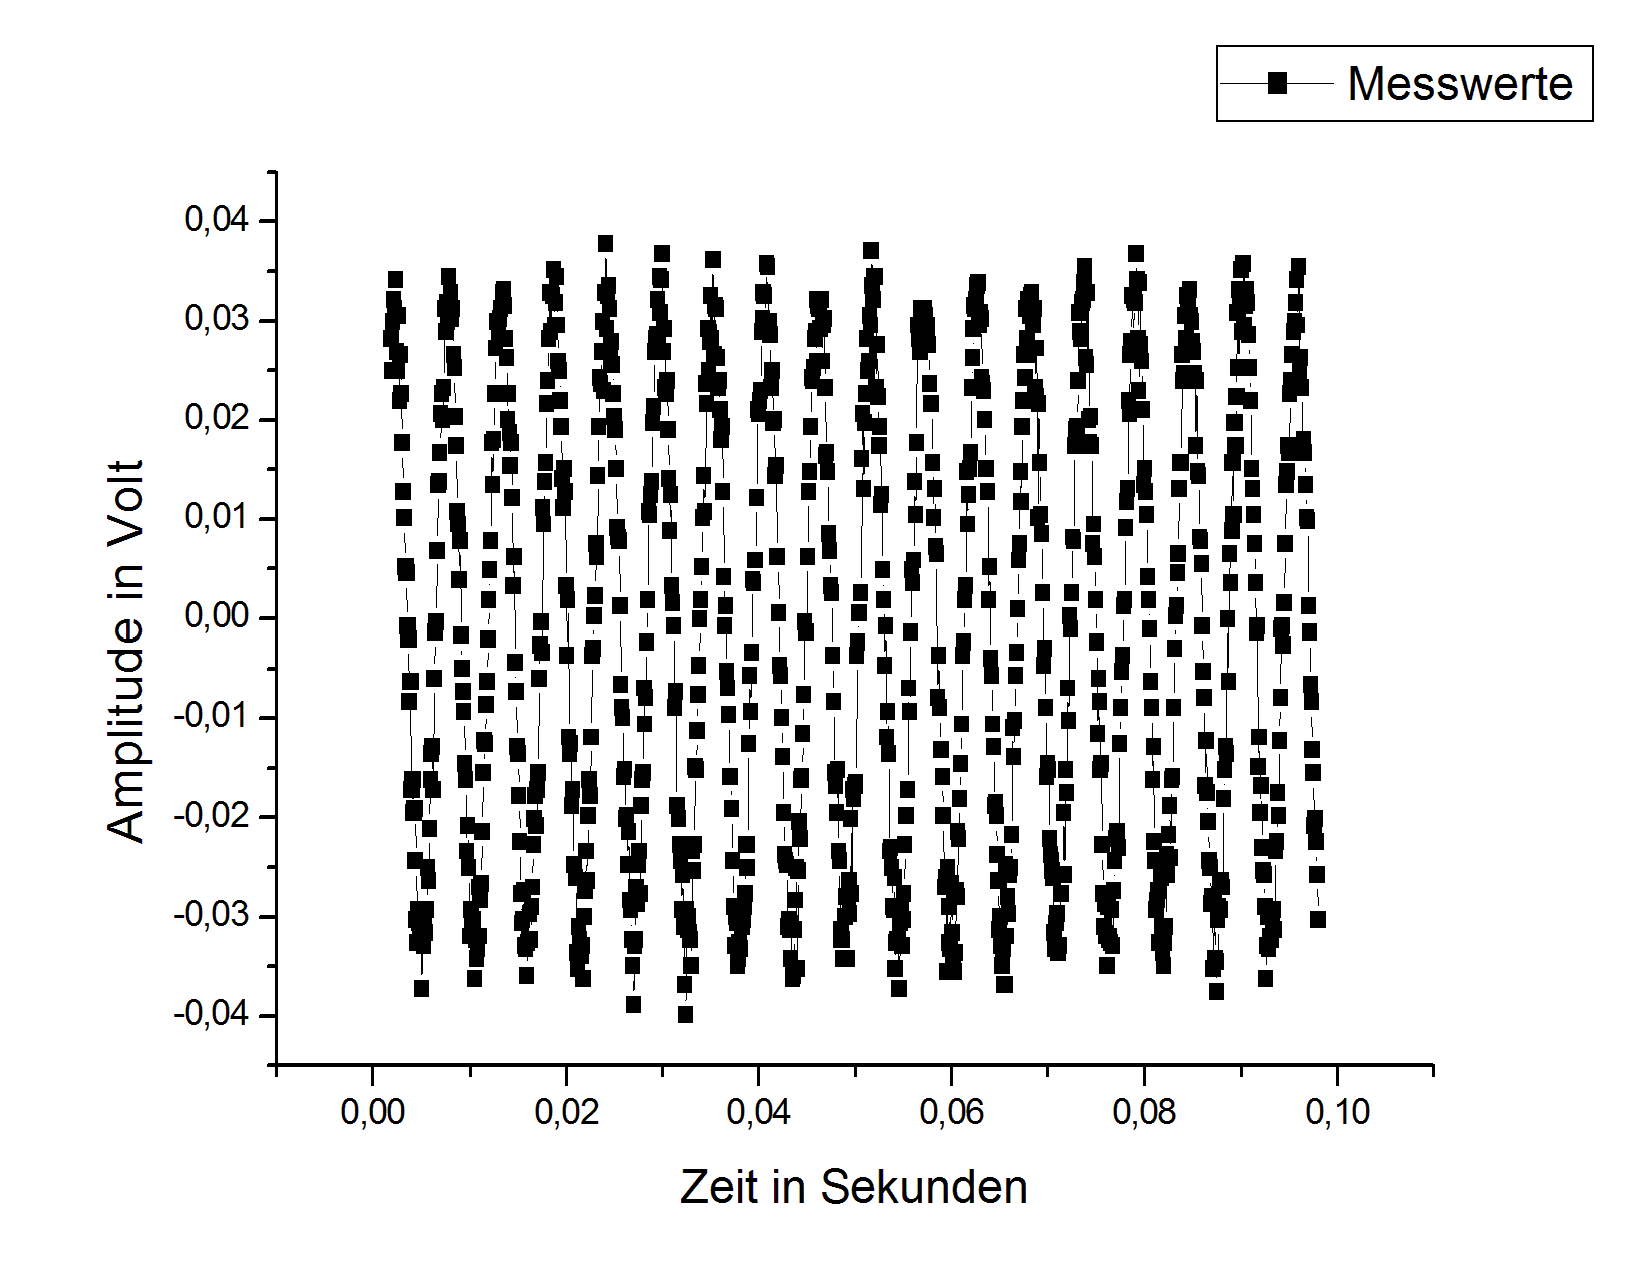
\includegraphics[scale=0.25]{SNR_1V_PP_Zeit}}
			\subfigure[Spektrum für $ U_{Rausch}^2 = $ \SI{8,1}{\milli\volt^2}]{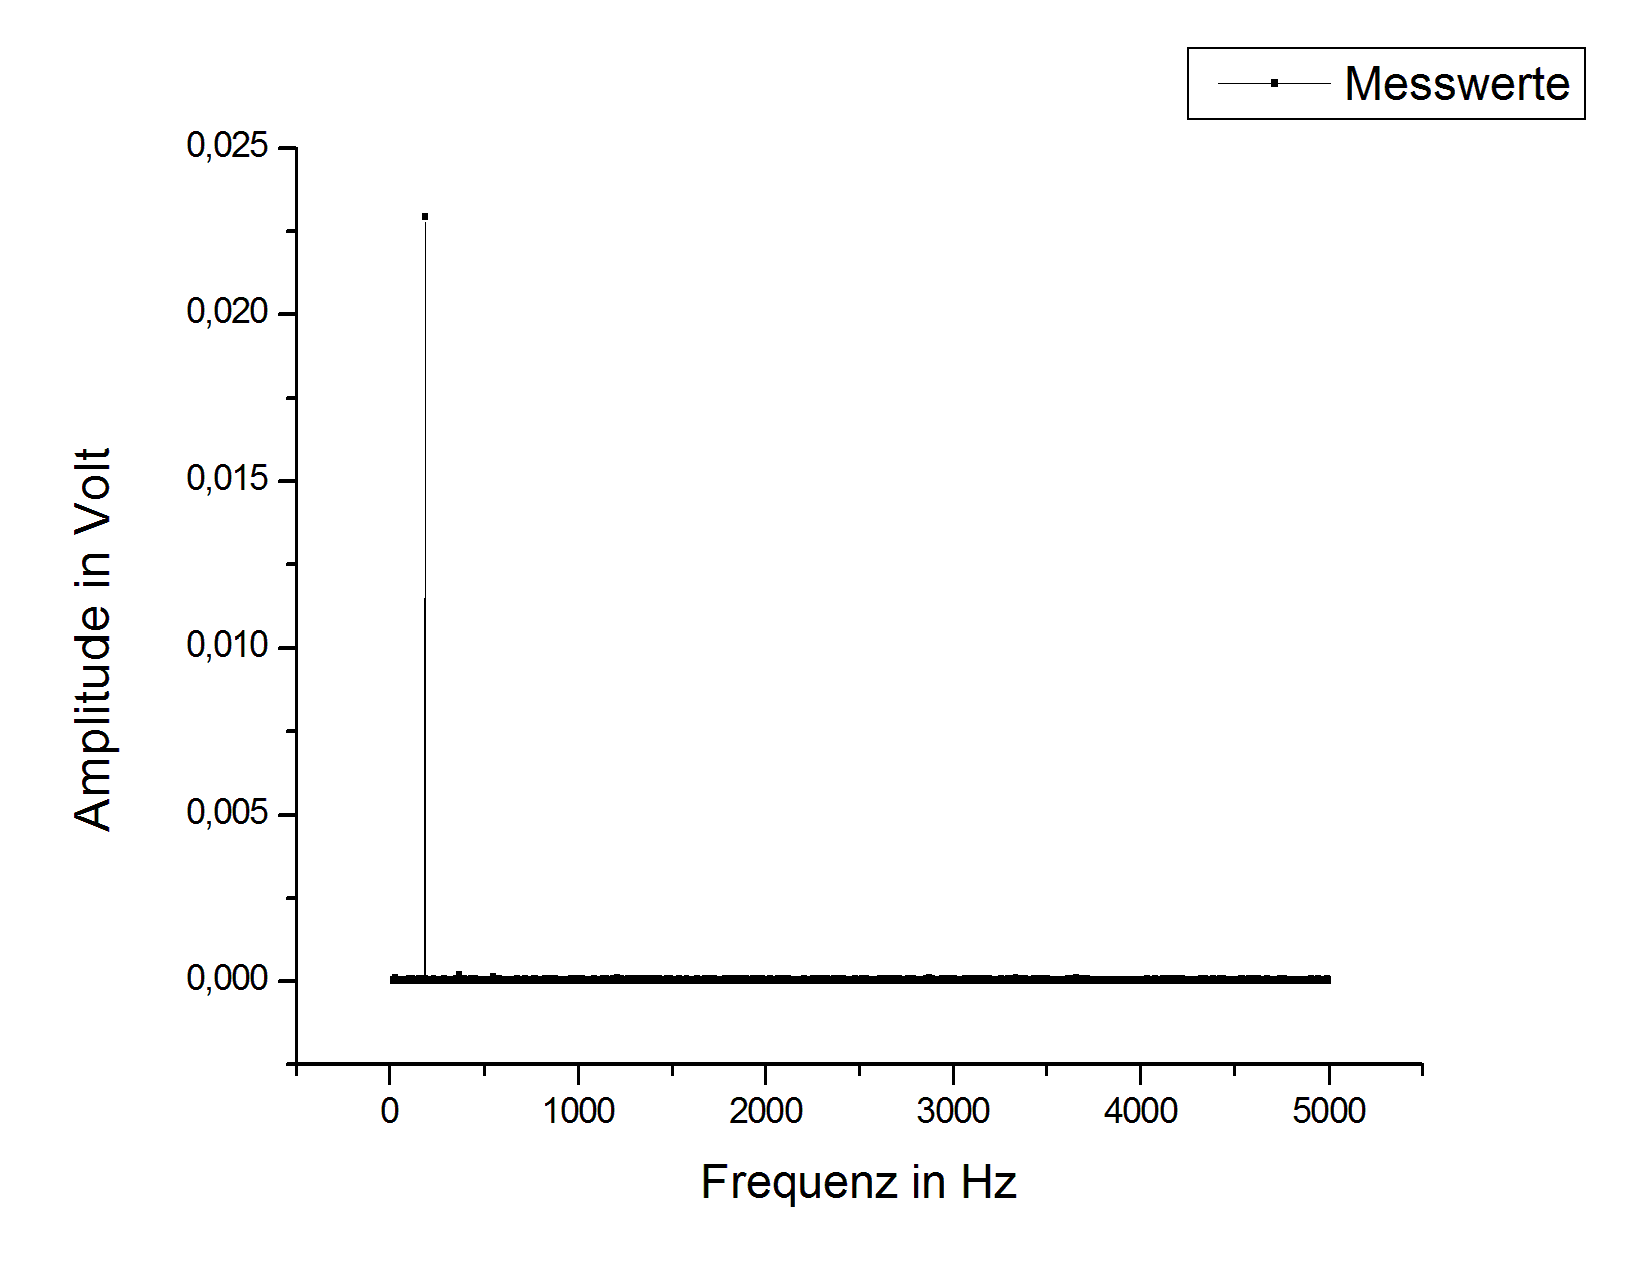
\includegraphics[scale=0.25]{SNR_1VPP_Frequenz}}
		\end{figure}
		
		\begin{figure}[h!]
			\caption{SNR=1,61}
			\subfigure[Zeitverlauf für $ U_{Rausch}^2 = $ \SI{3,22e-3}{\milli\volt^2}]{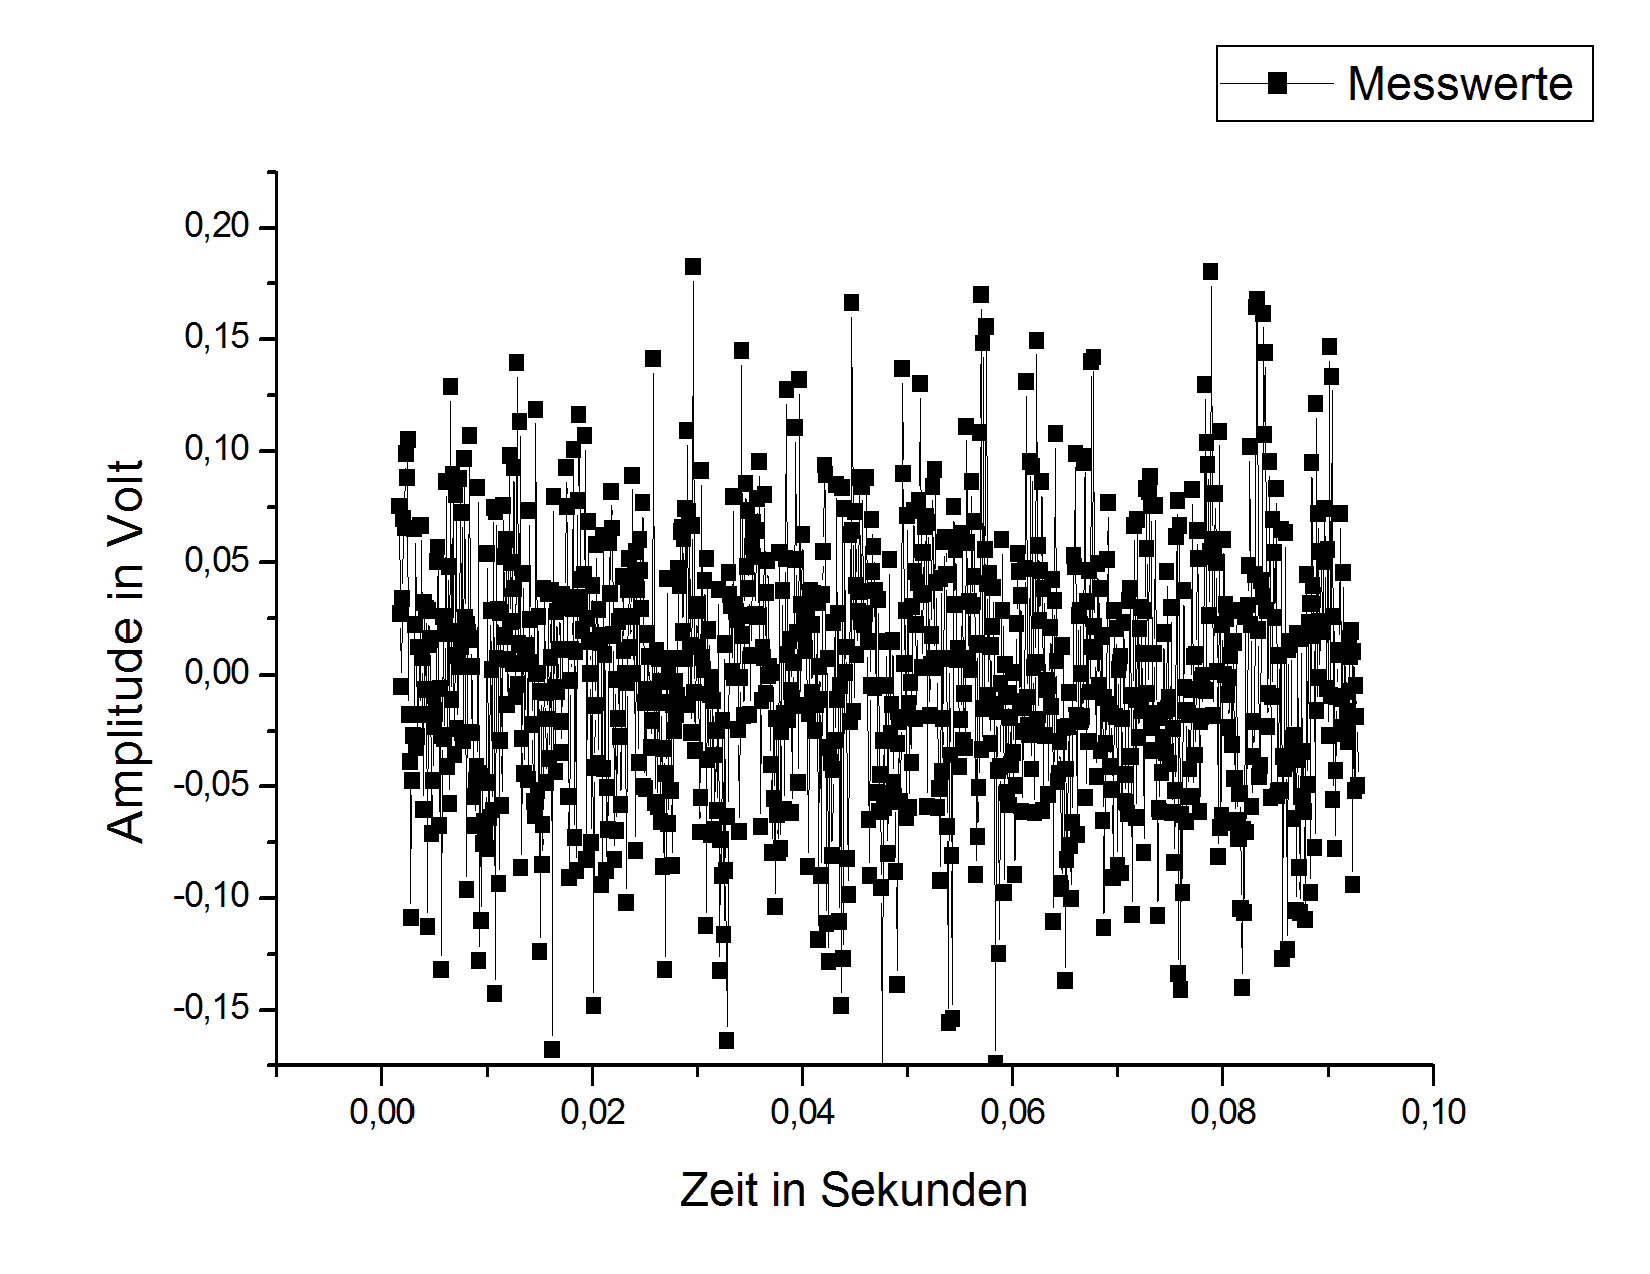
\includegraphics[scale=0.25]{SNR_20VPP_Zeit}}
			\subfigure[Spektrum für $ U_{Rausch}^2 = $ \SI{3,22e-3}{\milli\volt^2}]{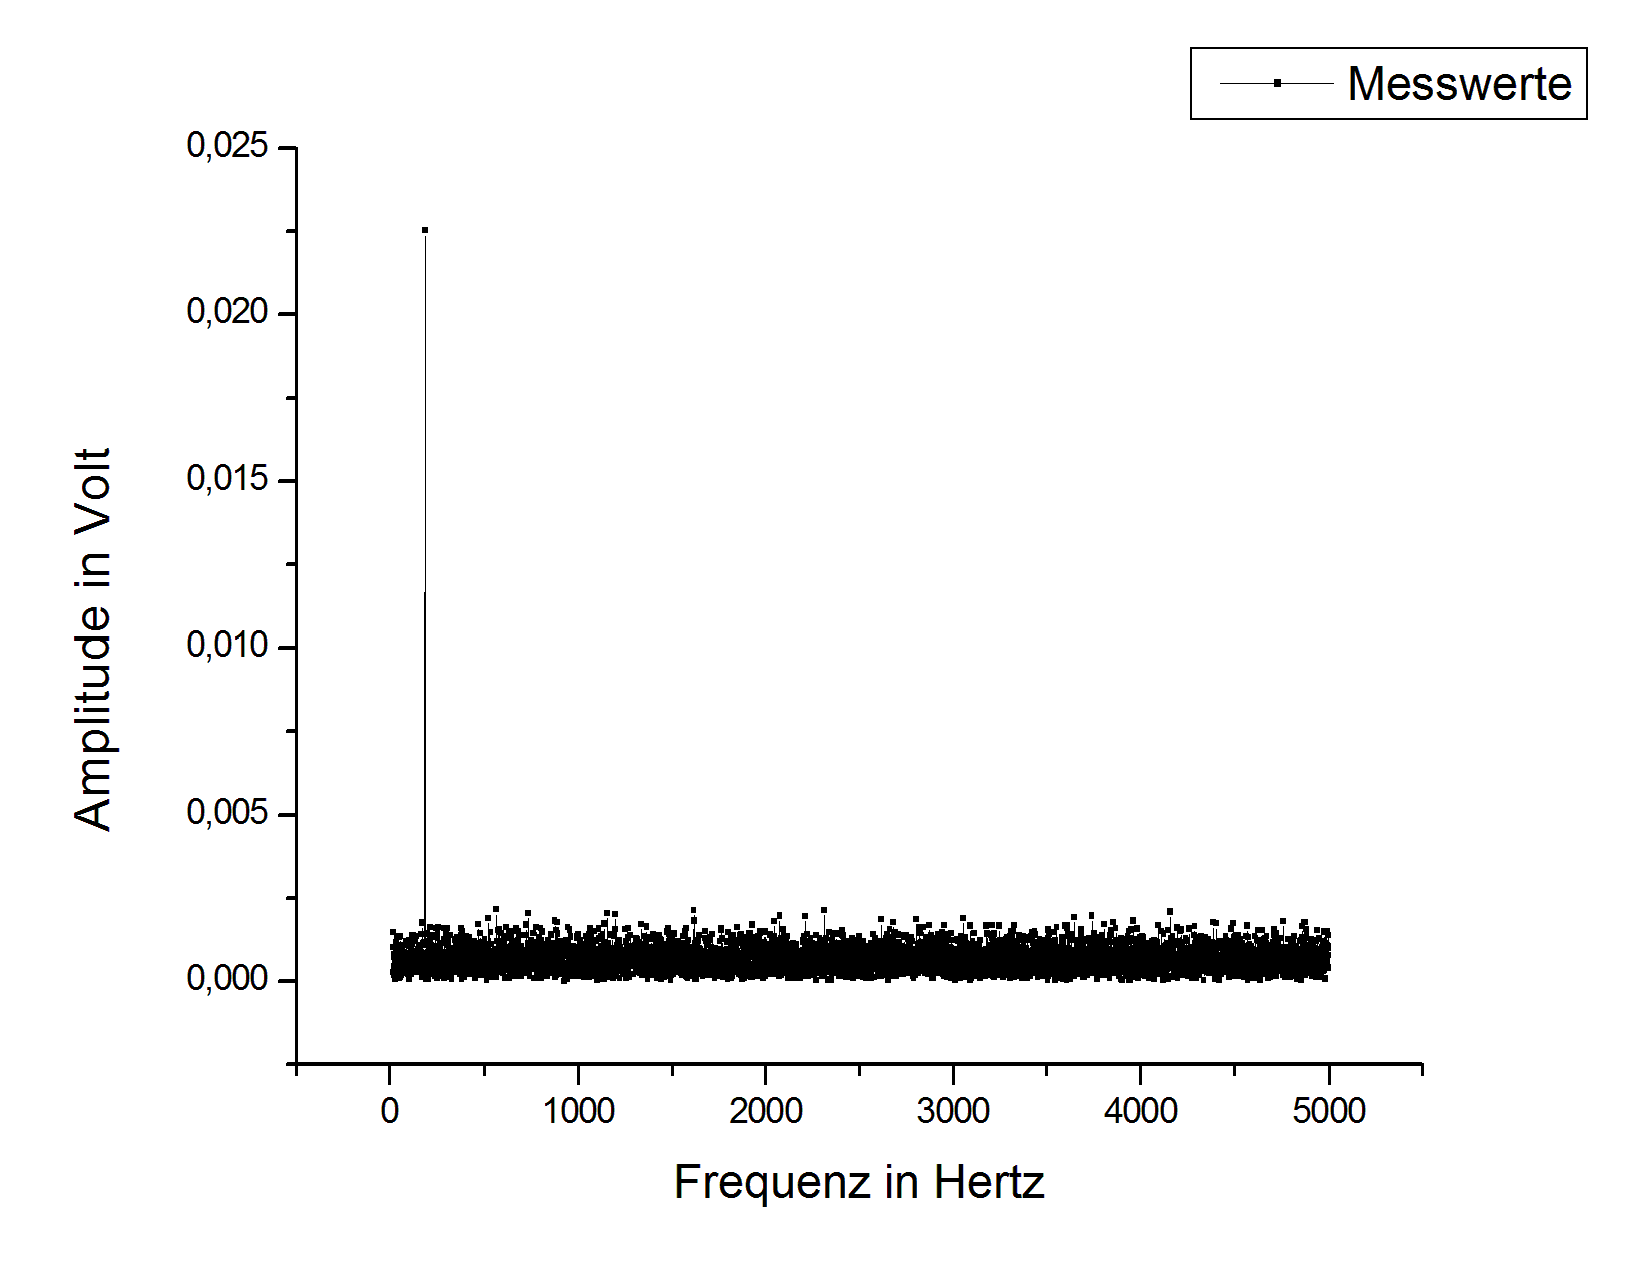
\includegraphics[scale=0.25]{SNR_20VPP_Frequenz}}
		\end{figure}
		\clearpage
		
		Im Aufgabenteil 1.2 ging es um die Rauschreduktion. Im Aufgabenteil 1.2 a) wurde dafür das Signal akkumuliert. Dies bedeutet, dass es mehrmals gemessen und dadurch gemittelt wurde. Als Beispiel hierfür wurde das Signal aus Aufgabenteil 1.1 e) verwendet mit einer Amplitude von $ U_{PP} = \SI{72}{\milli\volt} $ und einer Rauschamplitude von $ U^2 = \SI{7,95e-4}{\volt^2} $ und somit einem $ SNR = 6,5 $. Man erkennt eine deutliche Verbesserung durch die Akkumulation. Die Akkumulationstechnik hat jedoch zum Nachteil, dass die Messwertaufnahme länger dauert und dass diese nur funktioniert, wenn rauschen normalverteilt ist. 
		\begin{figure}[h!]
			\subfigure[Ohne Akkumulation]{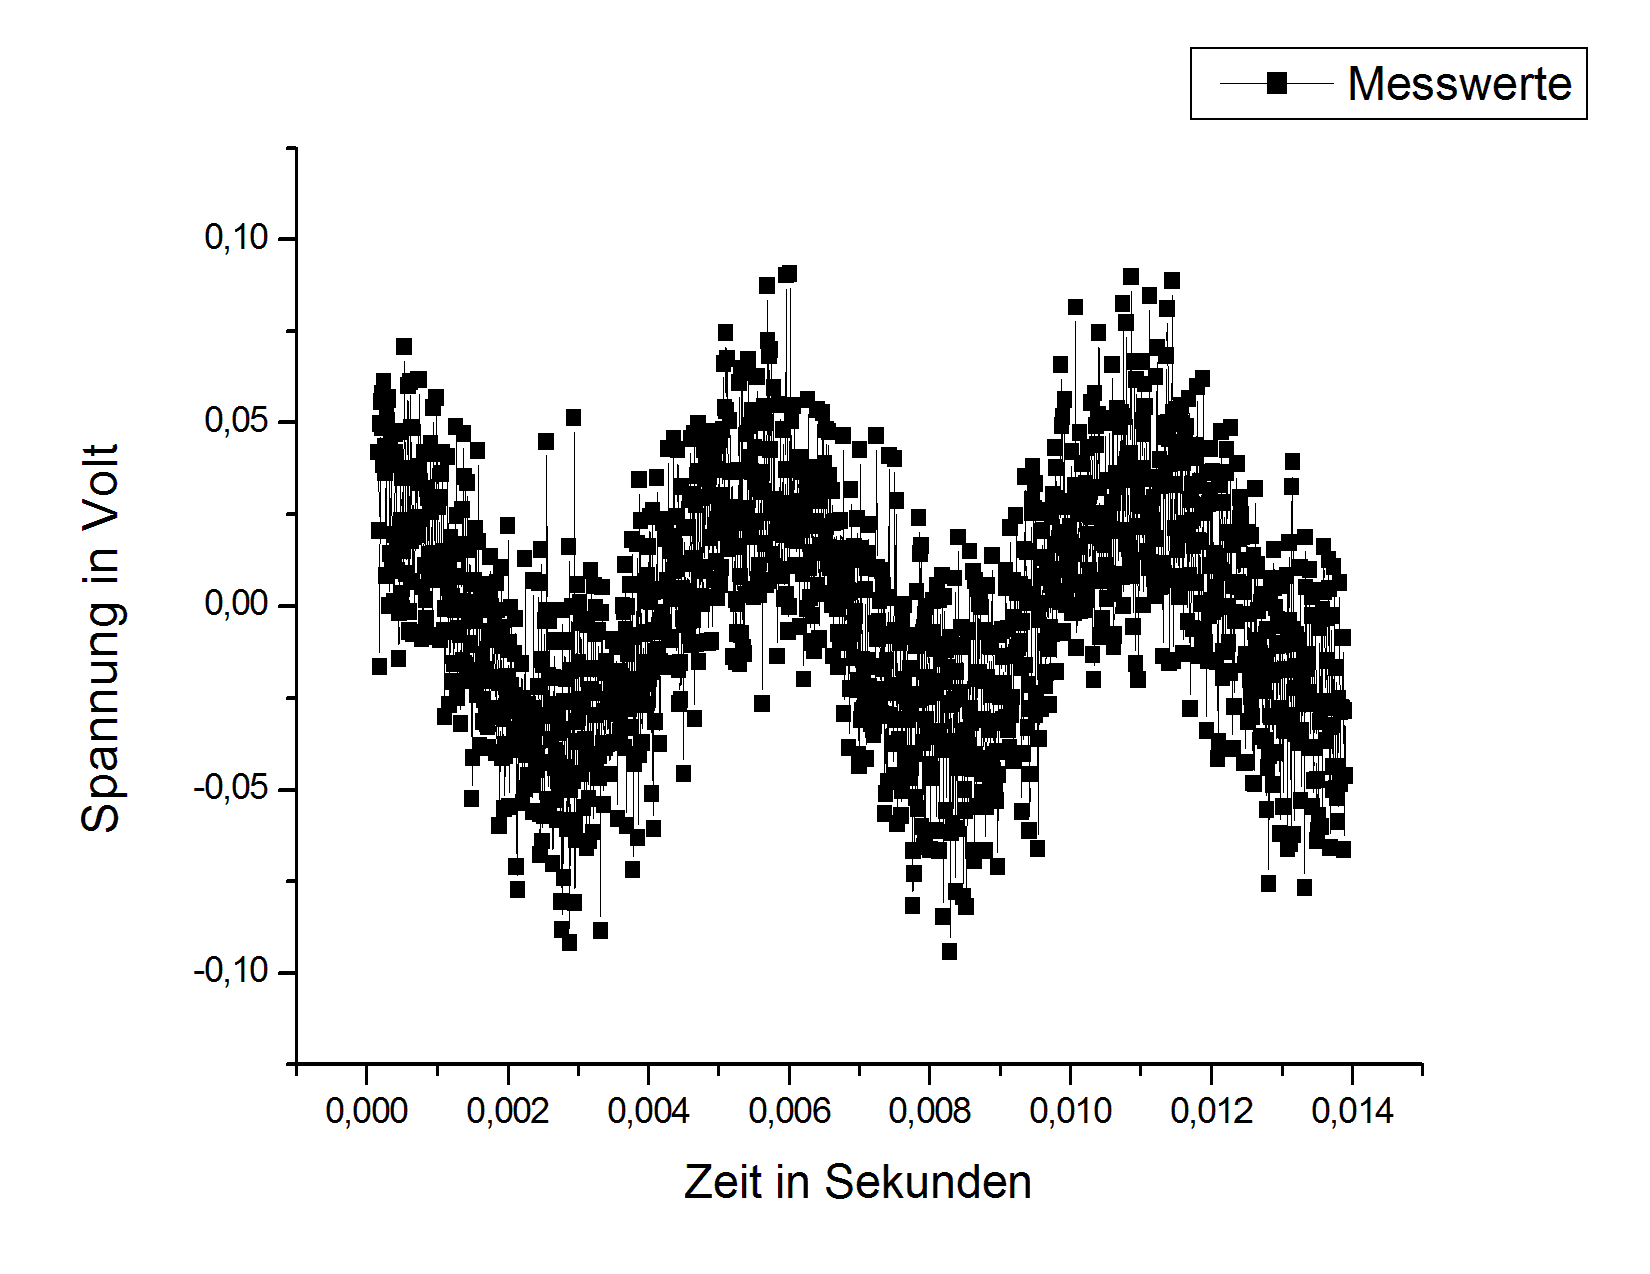
\includegraphics[scale=0.25]{Akkumulation1}}
			\subfigure[Mit 32-Facher Akkumulation]{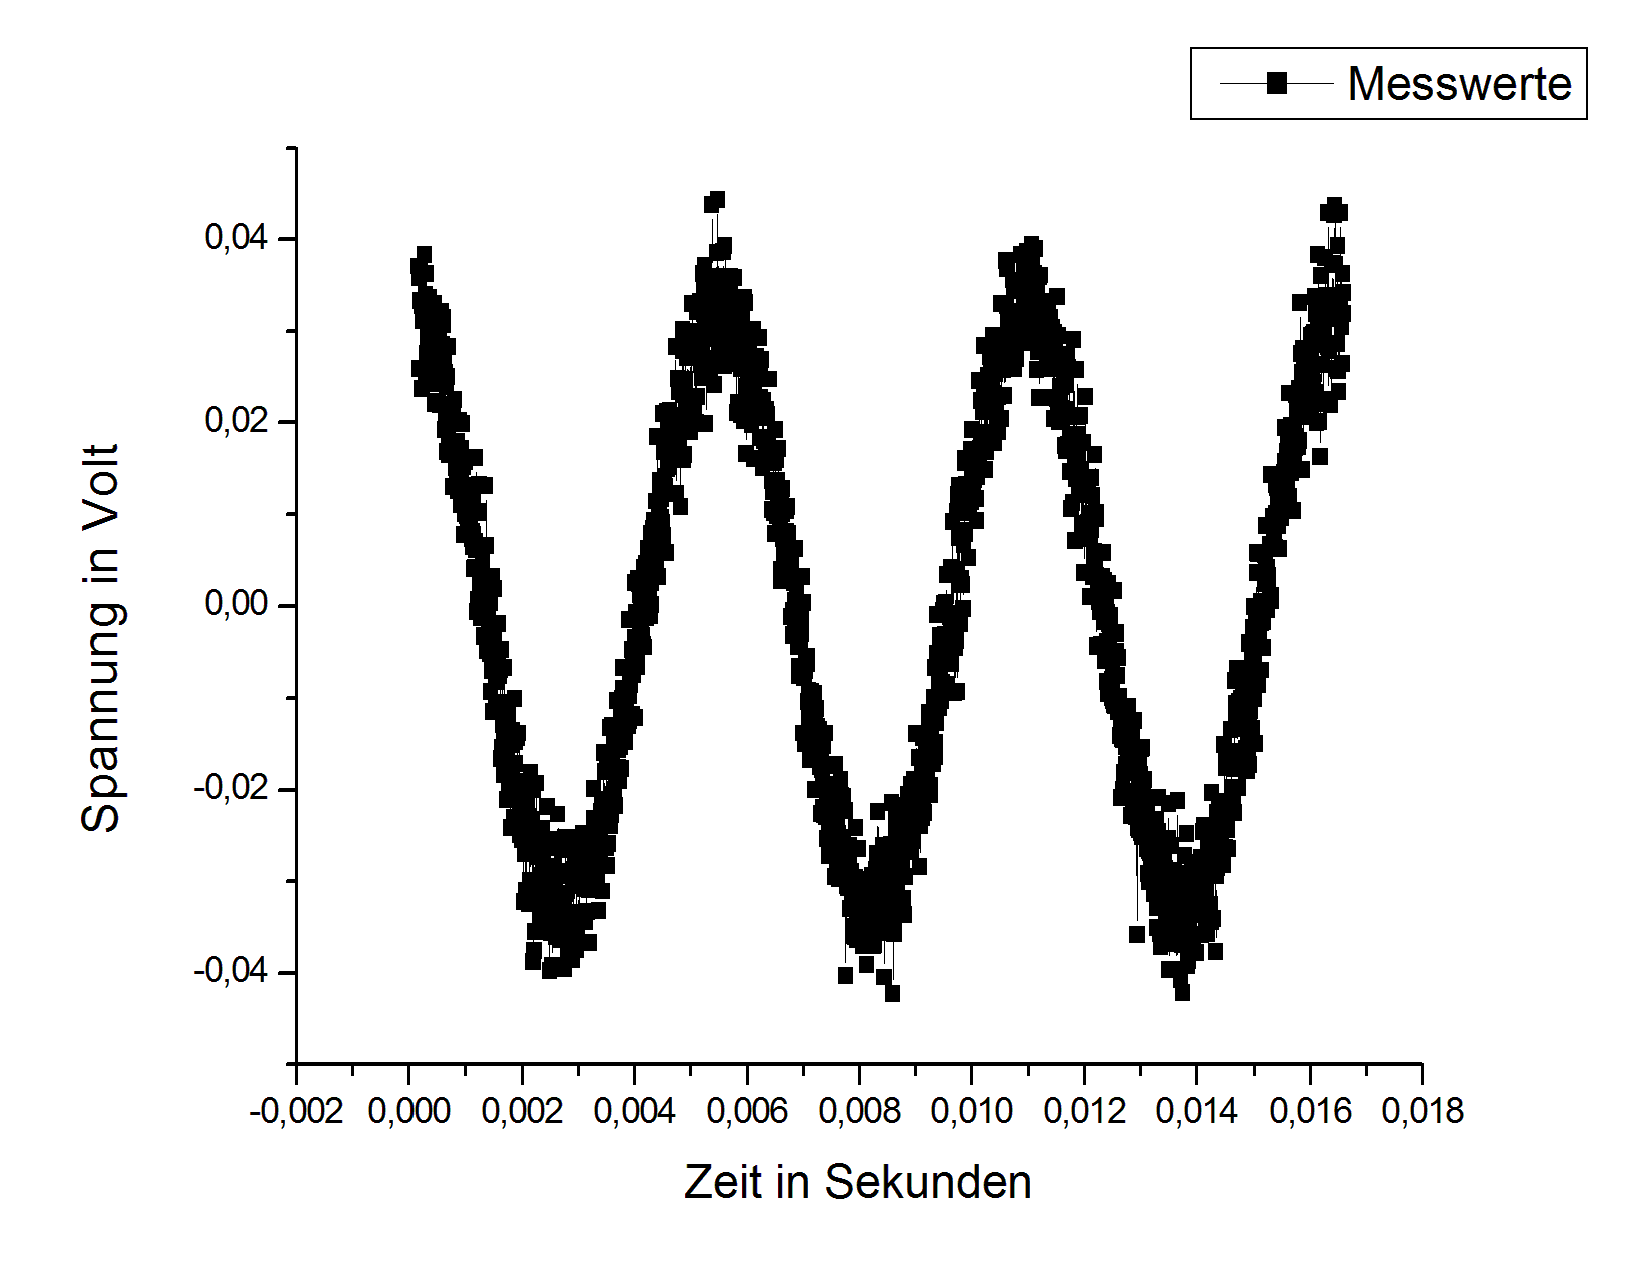
\includegraphics[scale=0.25]{Akkumulation32}}
		\end{figure}
		
		Als nächstes sollte in Aufgabe 1.2 b) der Tiefpass aus Aufgabe 1.1 verwendet werden und dadurch das Signal-/Rauschverhältnis verbessert werden. Dabei wurden die folgenden beiden Zeitverläufe aufgenommen. Es fällt dabei deutlich auf, dass das Rauschen bei dem Zeitsignal mit Tiefpass deutlich abgenommen hat im Vergleich zu dem Zeitsignal ohne Tiefpass. Dies liegt daran, dass durch den Tiefpass hohe Frequenzen weggefiltert werden und somit auch Rauschfrequenzen.
		
		\begin{figure}[h!]
			\subfigure[Ohne Tiefpass]{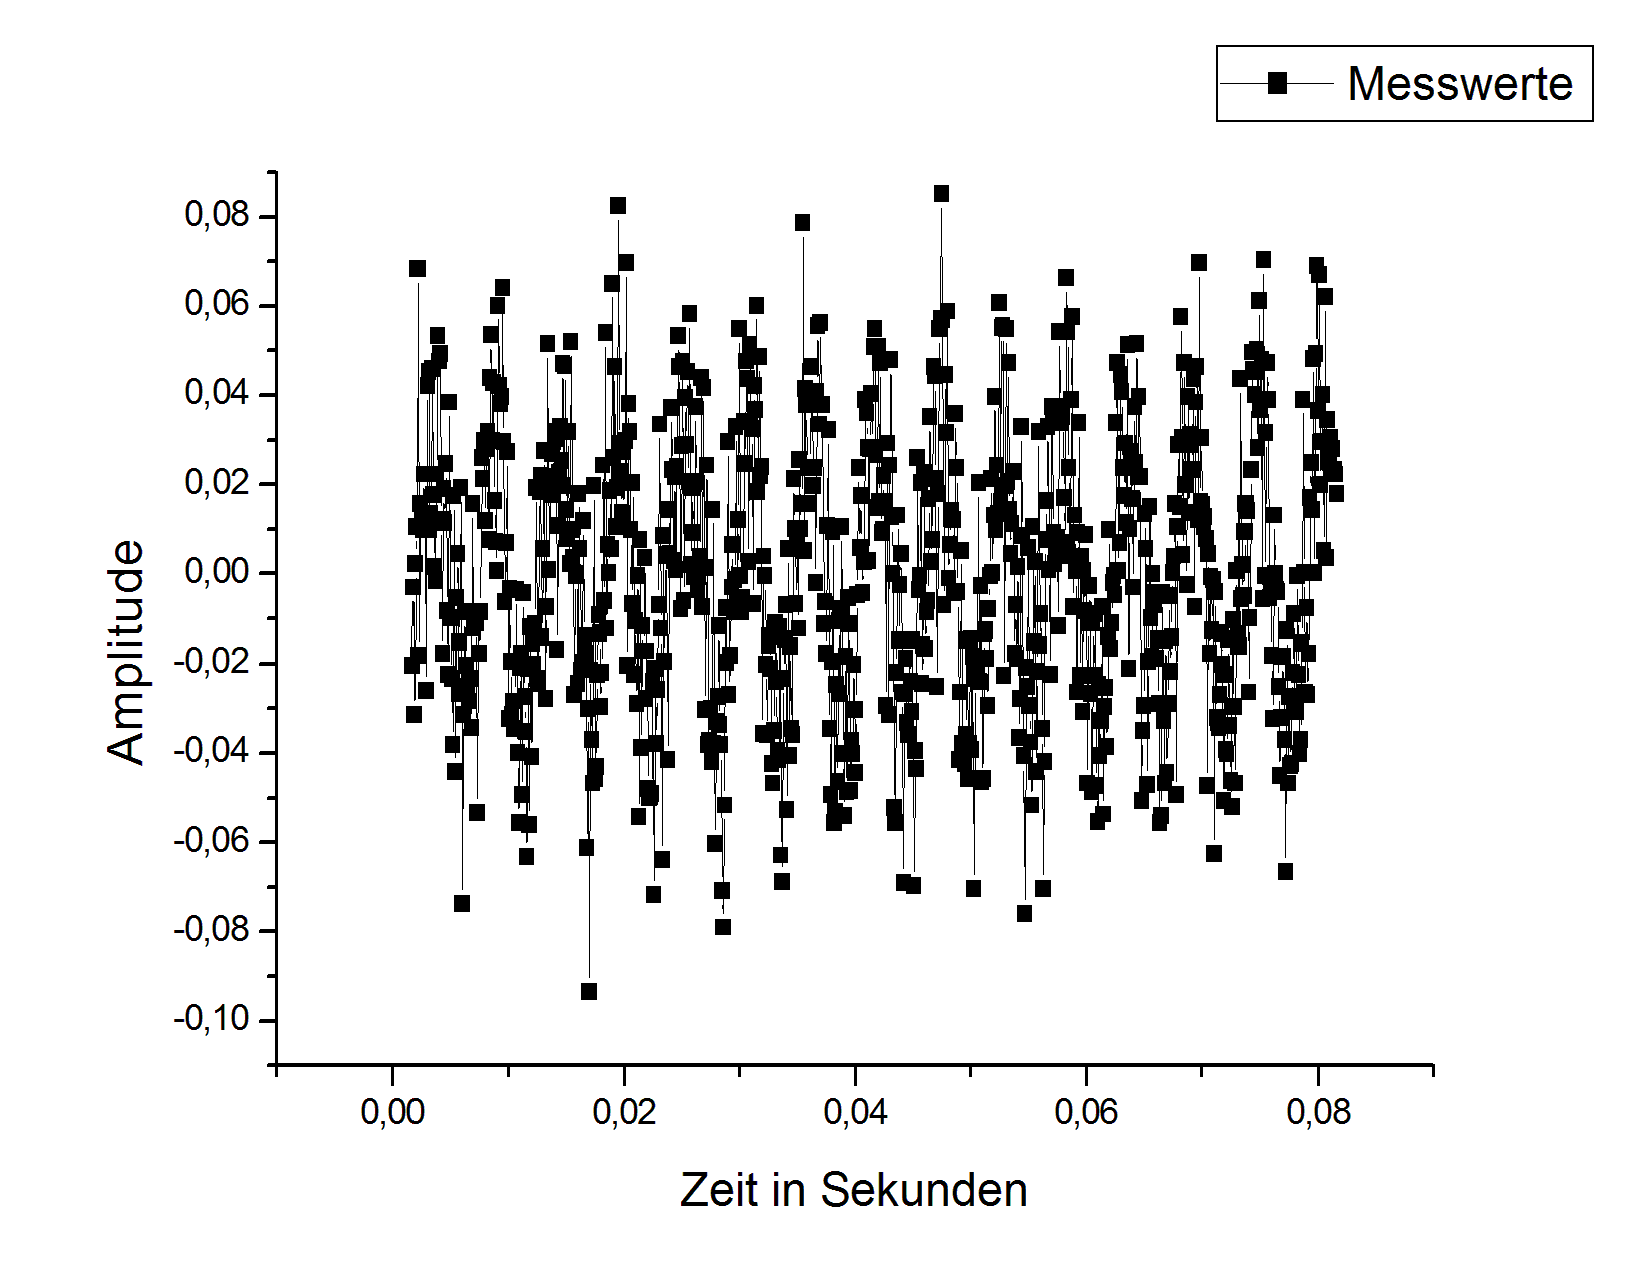
\includegraphics[scale=0.2]{OhneTiefoass_Zeit}}
			\subfigure[Mit Tiefpass]{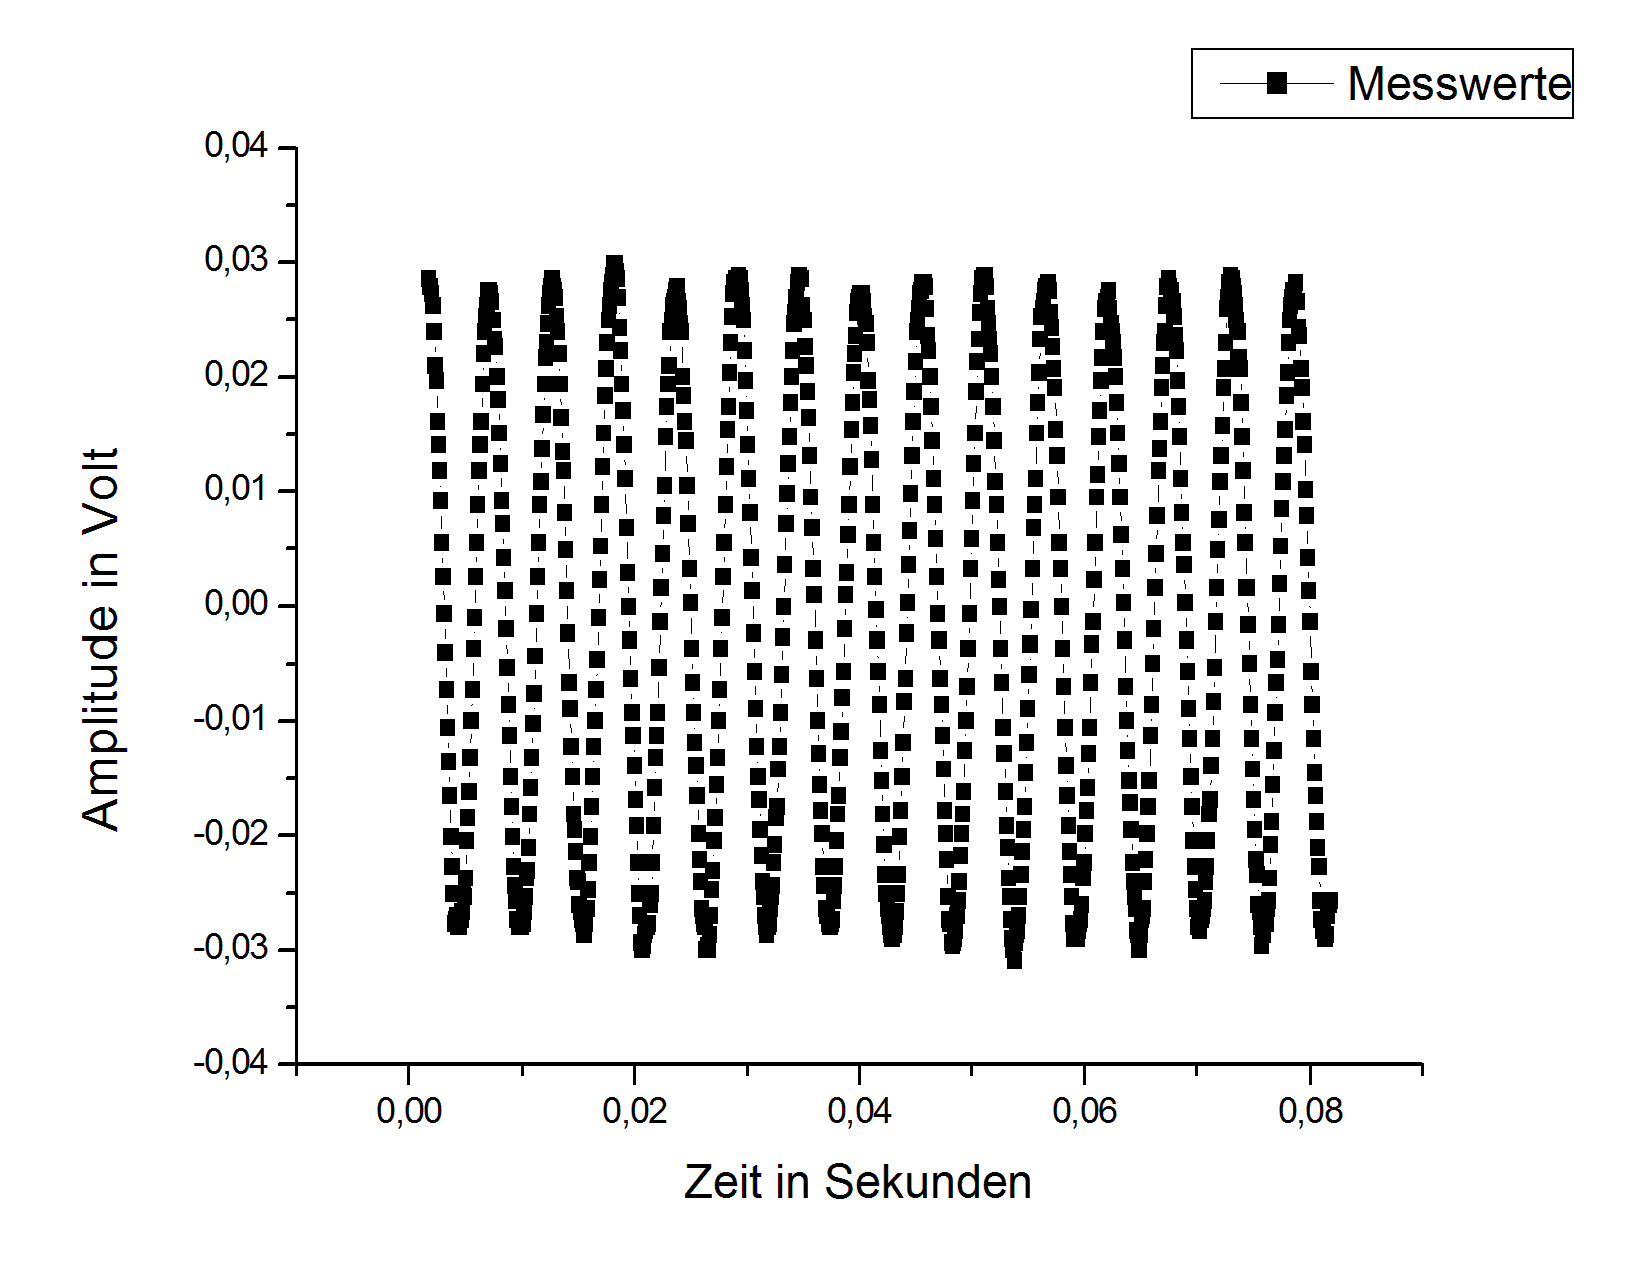
\includegraphics[scale=0.2]{MitTiefpass_zeit}}
		\end{figure}
		
		\clearpage
		
	\subsection{Auswertung Verstärkerrauschen}
		Am zweiten Tag ging es um das Verstärkerrauschen. Dafür sollten zunächst die Verstärkereigenschaften untersucht werden. In Aufgabe 1.1 sollte dafür die Amplitudenübertragungsfunktion des Verstärkers für eine Verstärkung von $ V = 10 $ und $ V = 1000 $ aufgenommen werde und aus den gewonnen Daten das Verstärkungs-Bandbreite-Produkt bestimmt werden. Danach sollte die Offsetspannung des Verstärkers ermittelt werde.
		
		Es wurden die folgenden beiden Übertragungsfunktionen aufgenommen:
		
		\begin{figure}[h!]
			\subfigure[V = 10]{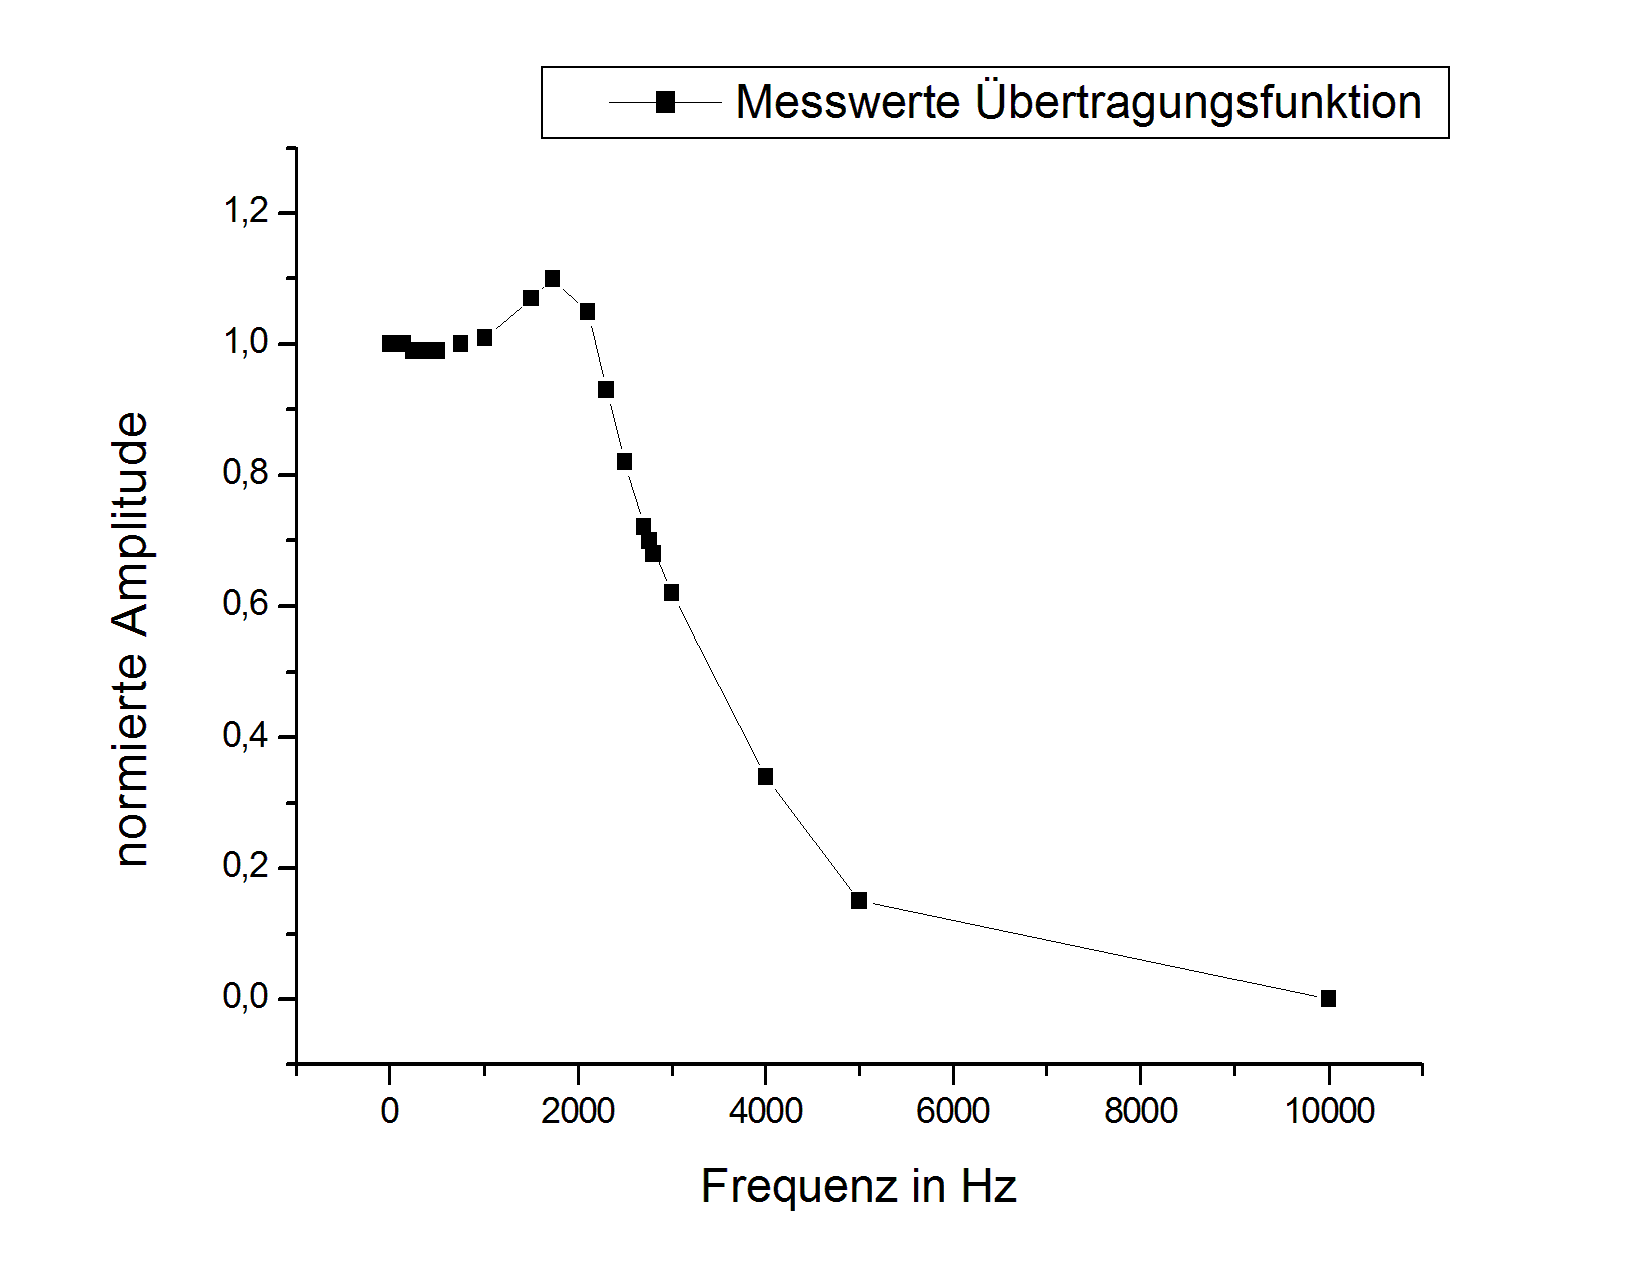
\includegraphics[scale=0.25]{UebertragungsfunktionV10}}
			\subfigure[V = 1000]{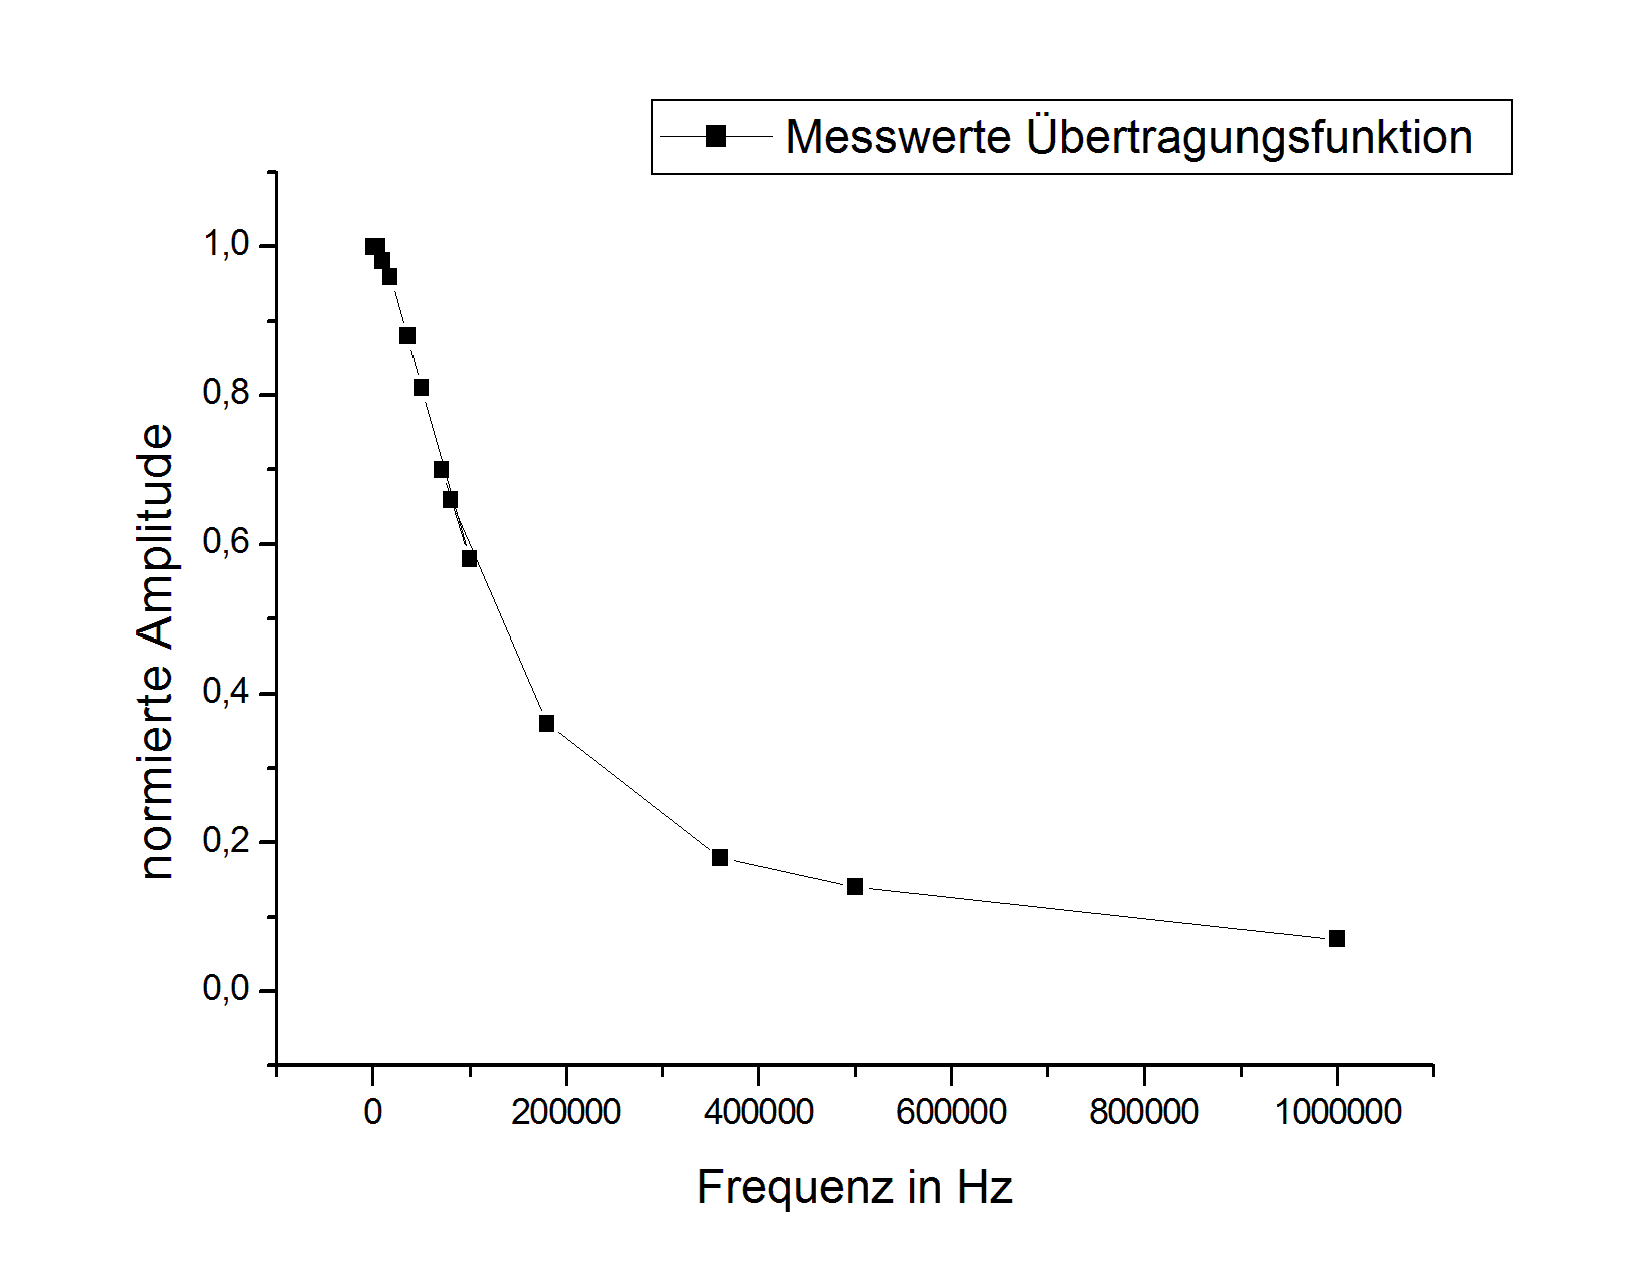
\includegraphics[scale=0.25]{UebertragungsfunktionV1000}}
		\end{figure}
		
		Aus den Übertragungsfunktionen kann man eine \SI{3}{\decibel} Bandbreite (Abfall auf $ \frac{1}{\sqrt{2}}) $ von $ B_{V=10} = \SI{2,75}{\mega\hertz} $ und $ B_{V=1000} = \SI{71}{\kilo\hertz} $ bestimmen.  Für das Produkt ergibt sich damit: $ P_{V=10}=\SI{27,5}{\mega\hertz} $ und $ P_{V=1000} = \SI{7,1}{\mega\hertz} $. Für die Offsetspannung wurde $ U_{V=10} = \SI{-1}{\milli\volt} $ und $ U_{V=1000} = \SI{-91}{\milli\volt} $ bestimmt. \\
		
		Im Aufgabenteil 1.2 sollte die Störanfälligkeit von hochohmigen und niederohmigen Quellen beobachtet werden. Dafür wurde der variable Quellwiderstand verwendet und verstärkt ans Oszilloskop angeschlossen.
		Für V = 10 und einen Vorwiderstand von R = \SI{1}{\giga\ohm} konnte am Oszilloskop ein Rauschen beobachtet werden. Wenn nun die Box des Widerstands mit der Hand berührt wurde, nahm das Rauschen zu. Wurde nun ein Widerstand von R = \SI{50}{\ohm} verwendet nahm das Rauschen merklich ab und durch eine Berührung mit der Hand konnte auch keine erkennbare Störung verursacht werden.
		
		Für eine Verstärkung von V = 1000 wurden die folgenden beiden Spektren aufgenommen: Dabei fällt wie bei der Verstärkung von V = 10 auf, dass es bei dem größeren Widerstand (R = \SI{100}{\kilo\ohm}) zu einem stärken Rauschen kommt. Man kann in beiden Spektren die Netzfrequenz von f = \SI{50}{\hertz} erkennen sowie dessen Oberwellen. Die Oberwellen nehmen mit zunehmender Frequenz ab.
		\clearpage
		
		\begin{figure}[h!]
			\subfigure[V = 1000 und ein Widerstand von R = \SI{50}{\ohm}]{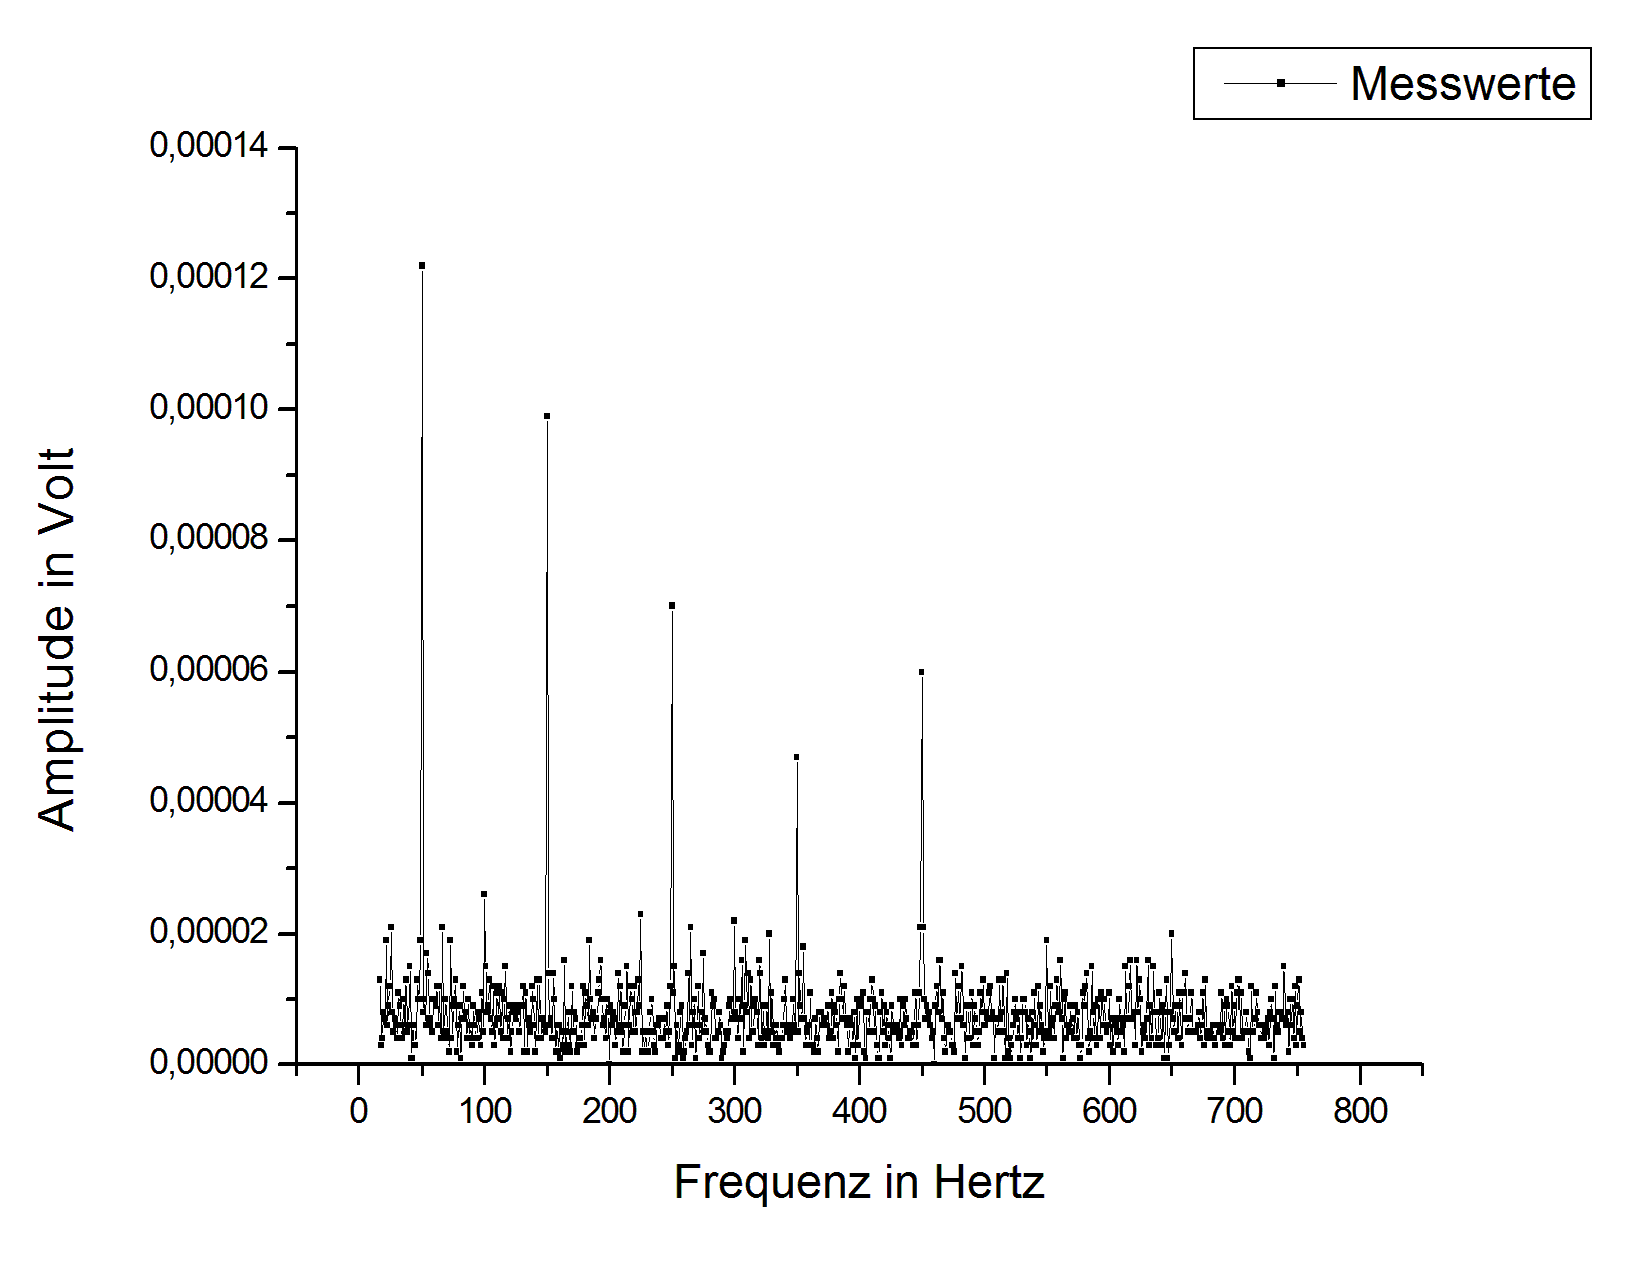
\includegraphics[scale=0.25]{Stoerung_Kleiner_Widerstand}}
			\subfigure[V = 1000 und ein Widerstand von R = \SI{100}{\kilo\ohm}]{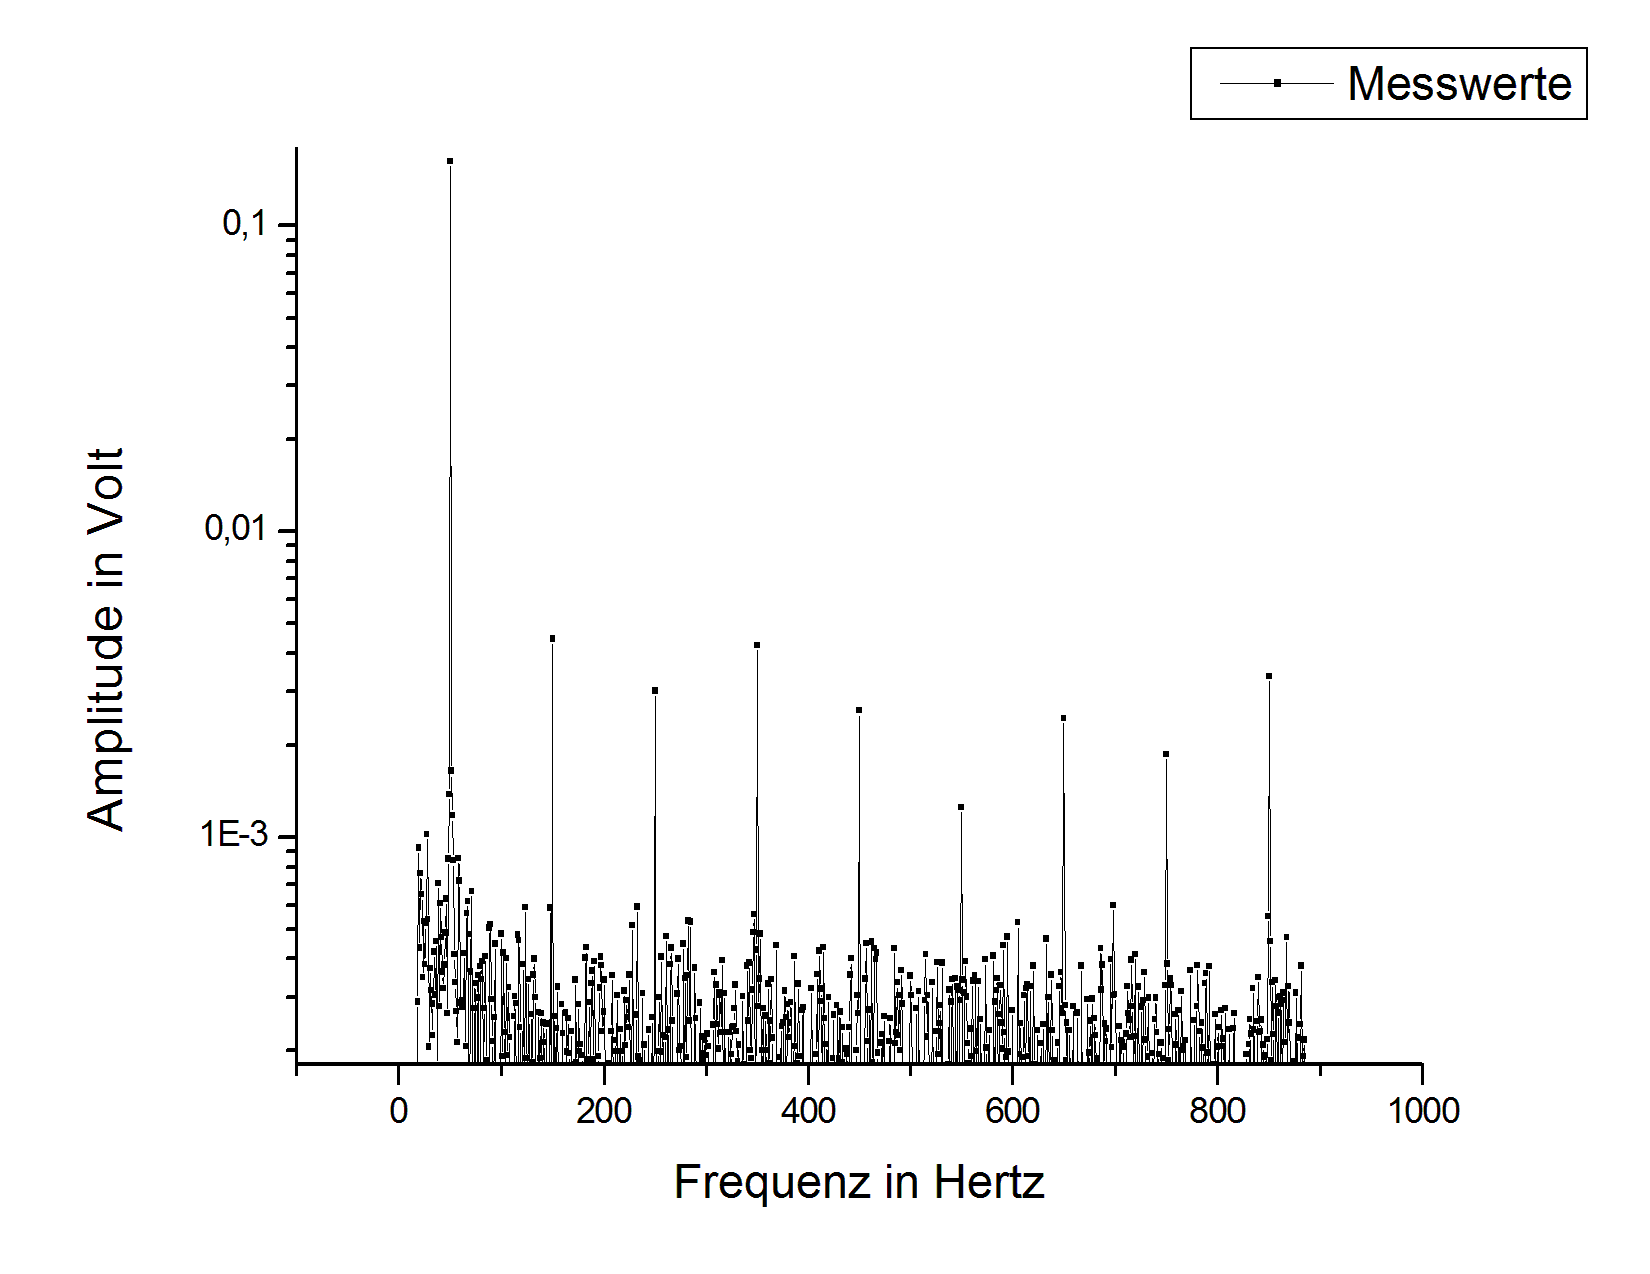
\includegraphics[scale=0.25]{Stoerung_Grosser_Widerstand}}
		\end{figure}
		
		Abschließend sollte in Aufgabe 1.2 die Wirkung einer Abschirmung untersucht werden. Dafür wurde wieder der Widerstand von R = \SI{100}{\kilo\ohm} verwendet. Durch die Abschirmung hat die Störanfälligkeit abgenommen. 
		
		\begin{figure}[h!]
			\centering
			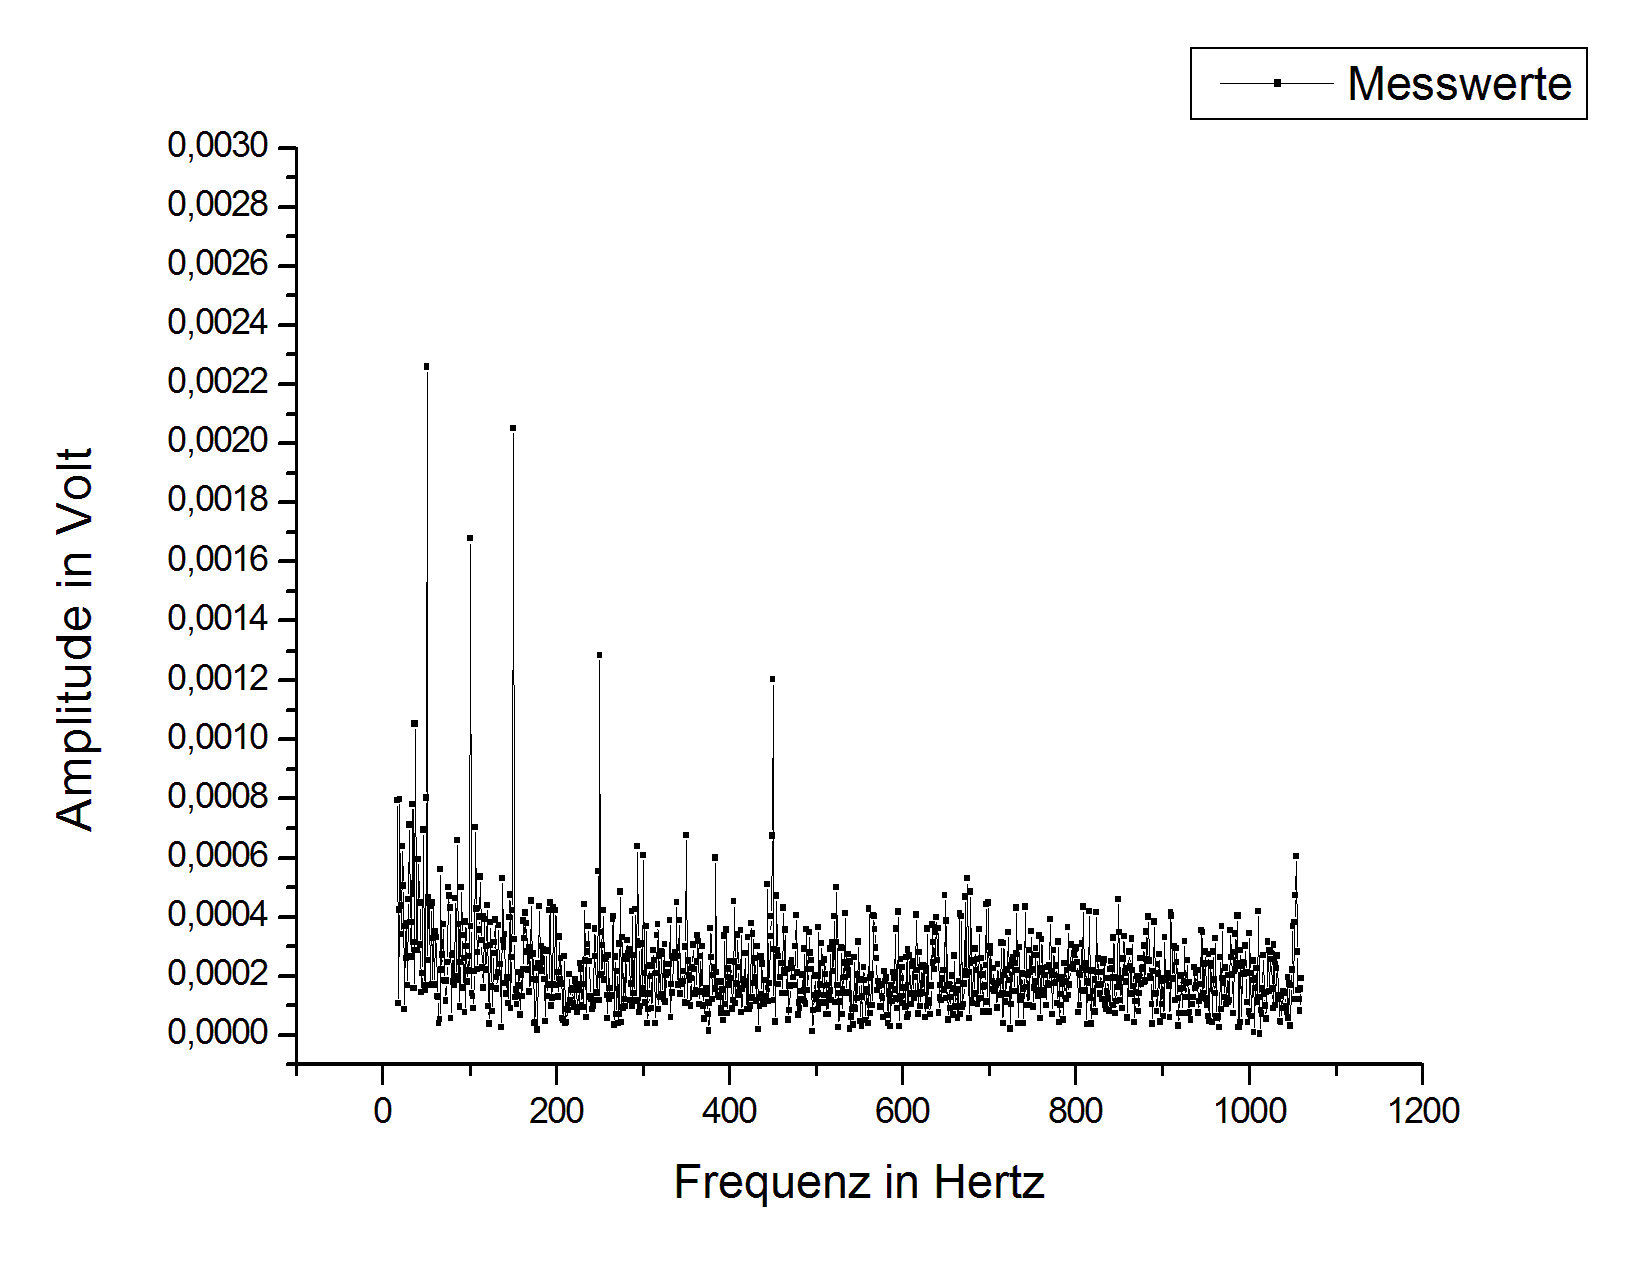
\includegraphics[scale=0.4]{Stoerung_mit_Abschirmung}
			\caption{V = 1000 und hochohmiger Widerstand}
		\end{figure}
		
		In der letzten Aufgabe 1.3 sollte das Verstärkerrauschen untersucht werden. Dazu wurde zunächst in Aufgabe 1.3 a) das Rauschspektrum des vorliegenden Verstärkers aufgenommen und auf $ \frac{1}{f} $ Rauschen untersucht. Dabei stellte sich heraus, dass kein $ \frac{1}{f} $ Rauschen für \SI{1}{\kilo\ohm} festgestellt werden konnte, jedoch für \SI{100}{\kilo\ohm} und einer Verstärkung von $ V = 1000 $. Dabei geht das $ \frac{1}{f} $ Rauschen an der Stelle $ f \approx \SI{70}{\hertz} $ in weißes Rauschen über. 
		
		\begin{figure}[h!]
			\subfigure[V = 1000 und R = \SI{100}{\kilo\ohm}]{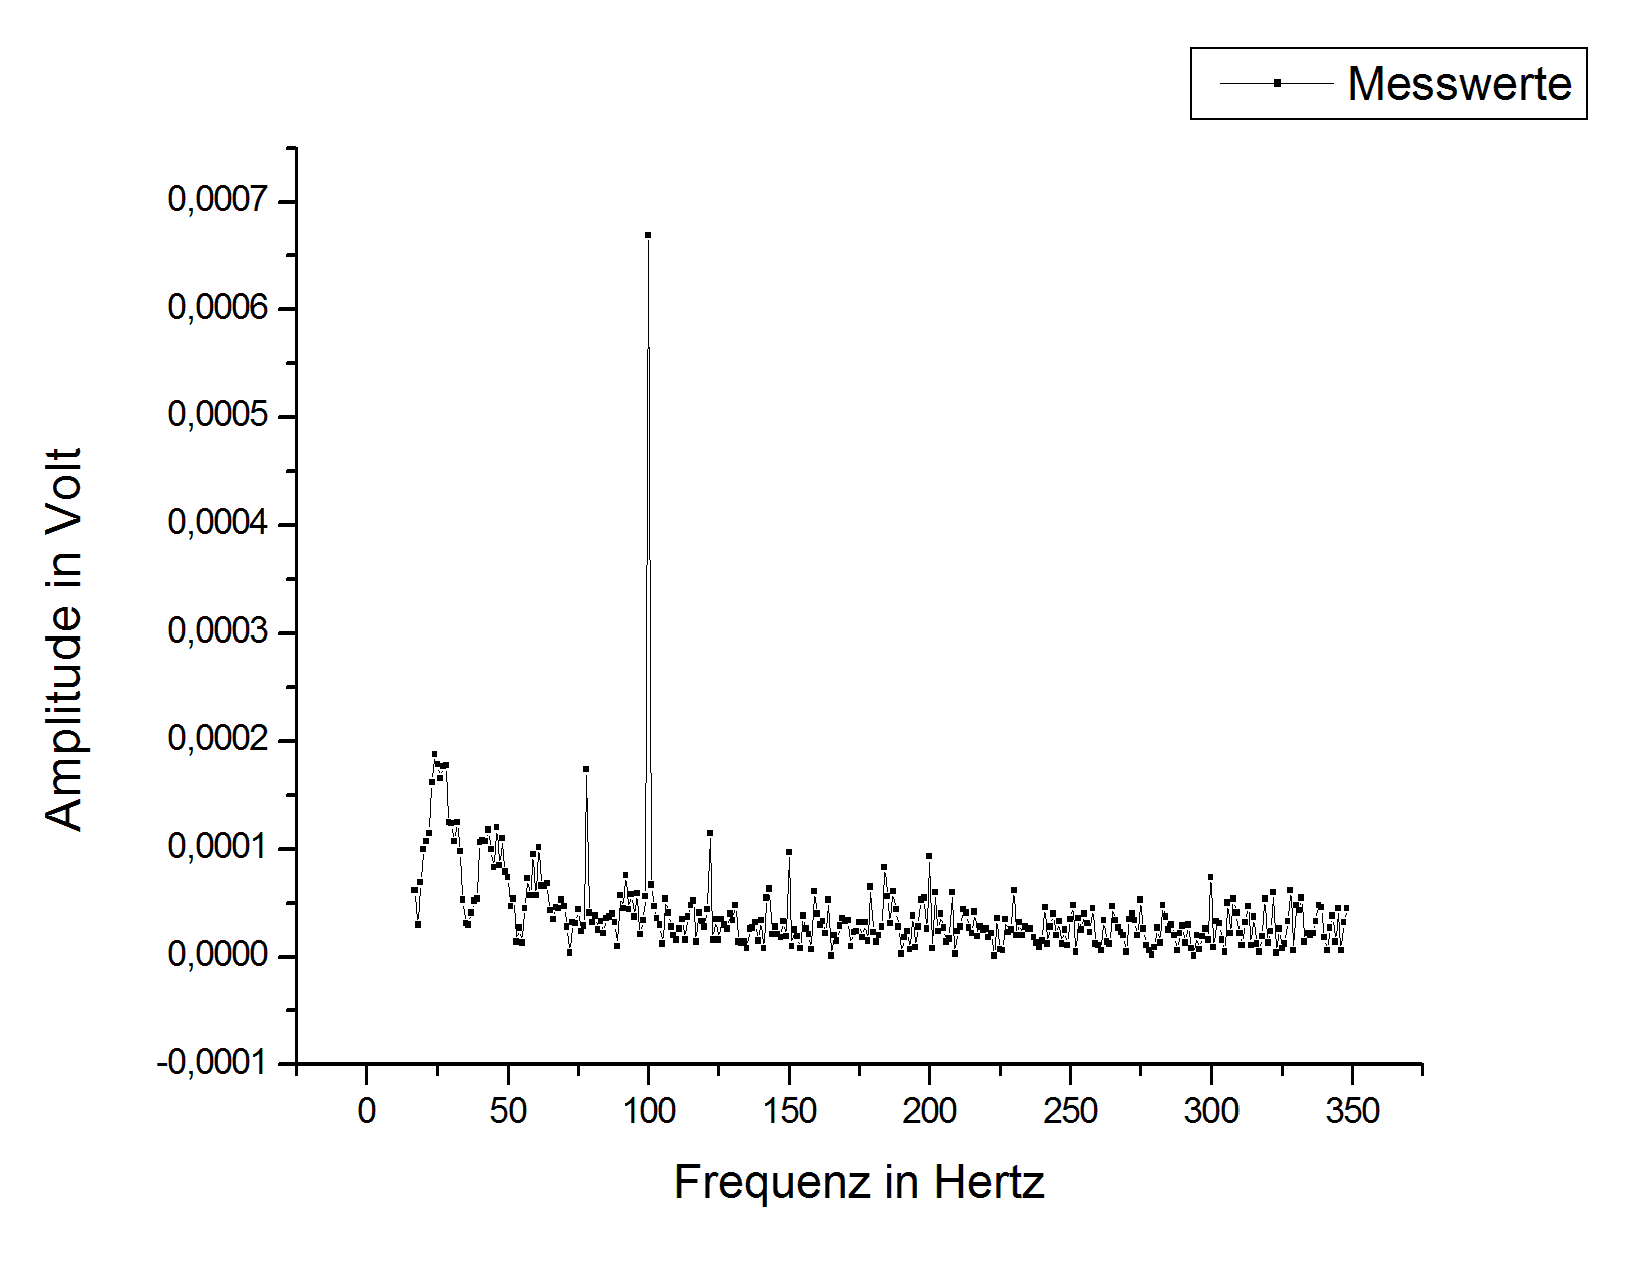
\includegraphics[scale=0.25]{1durchf_rauschen_V1000_100kiloOhm}}
			\subfigure[V = 1000 und R = \SI{1}{\kilo\ohm}]{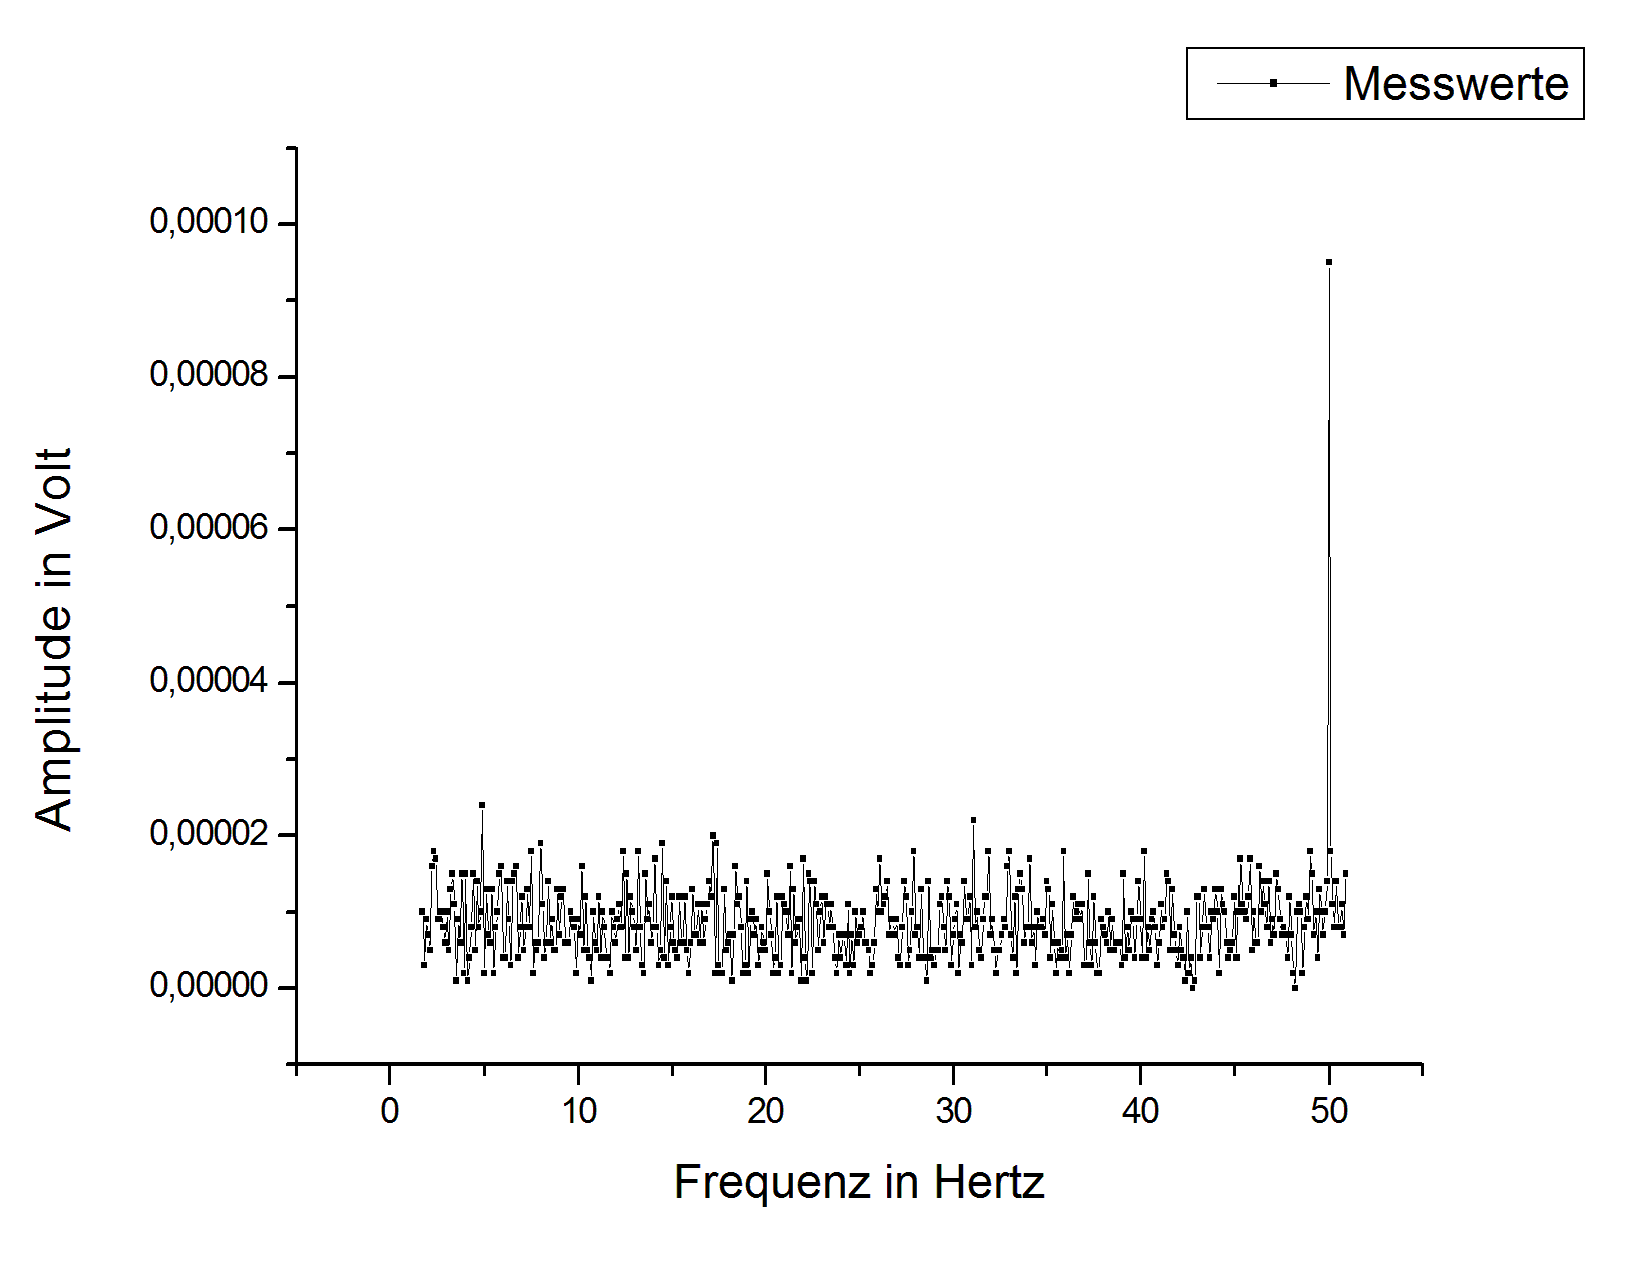
\includegraphics[scale=0.25]{1durchfRauschen_1kOhm_V1000}}
		\end{figure}
		
		Darauf folgend sollten die Rauschparameter bestimmt werden. Dafür wurde eine Messreihe mit Quellwiderstand, Mittelwert V und spektrale Rauschspannungsdichte angelegt und die spektrale Rauschspannungsdichte über den Widerstand aufgetragen. Aus diesem Graphen konnte man die Rauschparameter $ e_{n} $, $ i_{n} $ und $ R_{n} $ ablesen. Dabei ergibt sich: $ e_n = \SI{2,69e-6}{\frac{\volt}{\sqrt{\hertz}}} \hat{=} \SI{8,49e-8}{\volt}$. $ i_n $ kann man aus der Steigung der Tangente berechnen und ergibt: $ i_n = \frac{\Delta U}{\Delta R} = \frac{\SI{3,25e-7}{\volt}}{\SI{900}{\kilo\ohm}} = \SI{0,36}{\pico\ampere}$. Für Rauschanpassung wird gefordert: $ R_{opt} = \frac{e_n}{i_n} = \SI{236}{\kilo\ohm}  $
		
		\begin{figure}[h!]
			\centering
			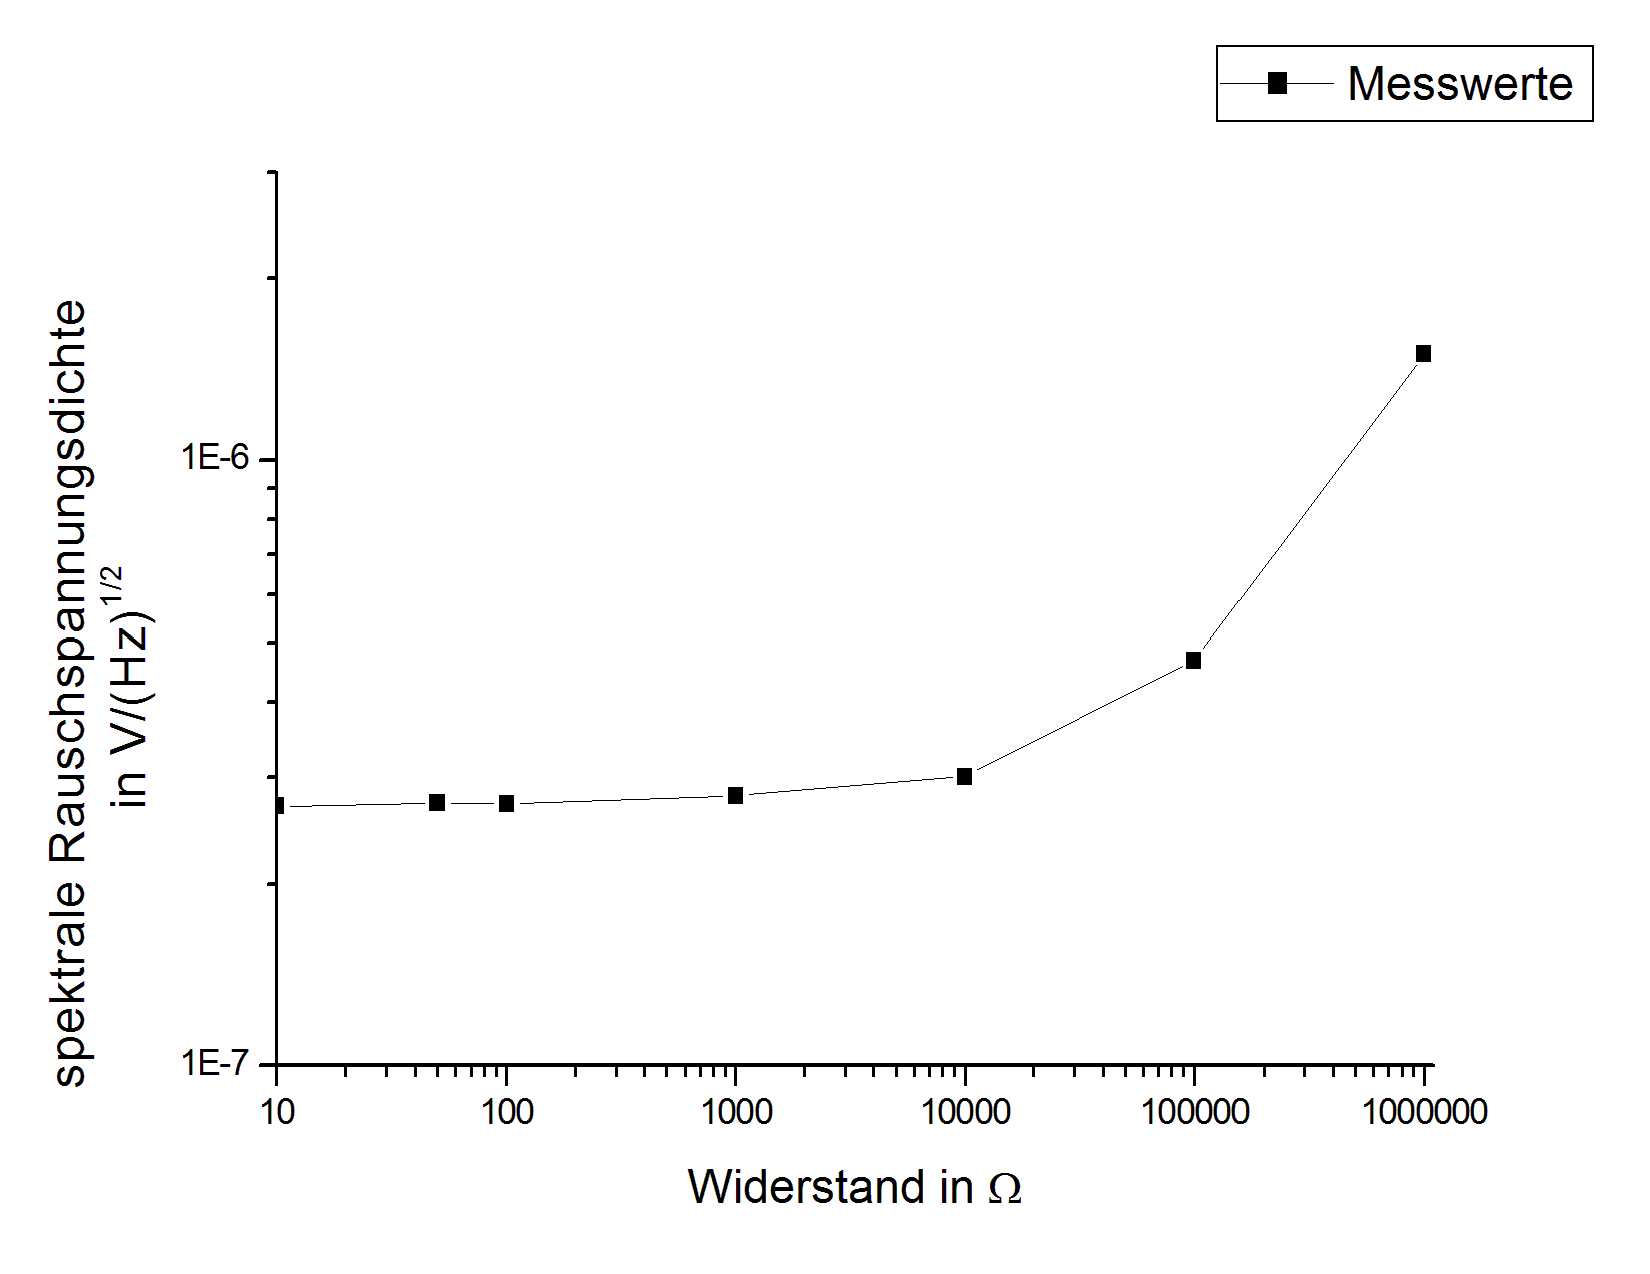
\includegraphics[scale=0.4]{EingangsbezogenesRauschen}
			\caption{Eingangsbezogenes Rauschen}
		\end{figure}
		
		\clearpage
\section{Diskussion}

	Grundsätzlich kann es bei den Messungen zu nicht abschirmbaren Störungen gekommen sein, wie z.B. magnetischen Einkoppelungen oder EM-Einstrahlungen. Diese hätten dann als systematische Fehler meine Messungen maßgeblich beeinflusst. Auch liefert z.B. beim Versuchsteil Rauschgrundlagen im Spektrum die Netzspannung einen 50Hz Peak sowie Oberwellen bei 150, 300Hz, sowie die Stromversorgung über einen Transformator den 100Hz Peak. [Diese sieht man leider in den obigen Diagrammen e), f) nicht, da das Frequenzintervall zu groß gewählt ist.] Bei der Autokorrelationsfunktion wurden unvollständige Messreihen aufgenommen (keine Werte für x>1, sodass die Richtigkeit des Verlaufes nicht garantiert werden kann. Ansonsten hatten wir große Probleme bei dem Verstärkerrauschen ein 1/f Rauschen einzustellen. Erst nach langem probieren, fanden wir die richtigen Einstellungen der Labview Software und der Verstärkung, um das erwartete 1/f Rauschen erkennen zu können (Bild a), letzte Seite der Auswertung). Erschütterungen des Versuchsaufbaus, Kontaktprobleme durch oxidierte Kabelspitzen oder Ladungen, welche von den Händen auf den Versuchsaufbau übertragen werden, können die Messungen zufällig verfälscht haben.
	

	
\section{Referenzen}
			\begin{itemize}
			\item Versuchsgrundlagen "Rauschgrundlagen-Anleitung.pdf" und "Verstärkerrauschen.pdf"
			\item zugehörige Tutorien  "Rauschgrundlagen-Tutorium.pdf" und "Verstärkerrauschen-Tutorium.pdf"
\end{itemize}				
\end{document}